\documentclass[11pt]{report}            %impostiamo il tipo di documento
%\documentclass[11pt]{scrreprt}         %alternativi, ha margini più larghi e altre minori differenze


%IMPORT PACKAGE & INIZIALIZZAZIONI & PERSONALIZZAZIONI PACKAGE- l'ordine ha importanza
%Compatibili input, output e lingua italiana
\usepackage[T1]{fontenc}                    
\usepackage[utf8]{inputenc}                 
\usepackage[italian]{babel} 
\usepackage{textcomp}

%Miglioramenti visivi - sempre necessario
\usepackage{microtype}                      

%Riferimenti intelligenti
\usepackage[italian]{varioref}              

%Gestione liste avanzata e semplificata
\usepackage[inline]{enumitem}           

%spazio vericale invece di indentazione nei paragrafi
%\usepackage{parskip}                       

%Gestione matematica
\usepackage{amsmath, amsthm, amssymb}   

%gestione indice analitico
\usepackage{makeidx}                        
\makeindex

%Gestione inserimente di codice
\usepackage{listings}

%Gestione tabelle avanzata
\usepackage{booktabs}           
\usepackage{longtable}      
\usepackage{tabularx}
\usepackage{multirow}
\usepackage{multicol}

%gestione delle immagini e dei colori
\usepackage[dvipsnames]{xcolor}
\usepackage{soulutf8}   
\usepackage{graphicx}   
\usepackage{rotating}
\usepackage{pdflscape}

                    %Inserire le immagini  dim relative a \textwidth
                    %es: 0.8\textwidth
                
%Gestione figura con sottofigura
\usepackage{subfig}     

%Gestione avvolgimento figure dal testo
\usepackage{wrapfig}    

%Gestione didascalie avanzata
\usepackage{caption}
\captionsetup{tableposition=top,figureposition=bottom,font=small,format=hang,labelfont={sf,bf}}

%Gestione didascalie a lato di una figura
\usepackage{sidecap}

%Gestione date
\usepackage{datetime}

%Miglioramento quoting                      
\usepackage{quoting}
\quotingsetup{font=small}

%Permette i commenti
\usepackage{comment}

%Gestione grafici
%\usepackage{pgfplots}
%\pgfplotsset{/pgf/number format/use comma,compat=newest}

%Gestione unità di misura
\usepackage[output-decimal-marker={,}]{siunitx}
                    %Per inserire numeri va usato \num{...}
    
%Gestione bibliografia e citazioni
\usepackage[autostyle,italian=guillemets]{csquotes}
\usepackage[backend=biber,style=philosophy-modern]{biblatex}
\addbibresource{bibliografia/bibliografia.bib}  %estensione necessaria (unico caso!)

%Roba per il titolo (strumenti grafici) 
\usepackage{tikz}
\usepackage{epigraph}
 
%Gestione dei link
\usepackage{hyperref}   
\hypersetup{
%   bookmarks=true,         % show bookmarks bar?
%   unicode=false,          % non-Latin characters in Acrobat’s bookmarks
%   pdftoolbar=true,        % show Acrobat’s toolbar?
%   pdfmenubar=true,        % show Acrobat’s menu?
%   pdffitwindow=false,     % window fit to page when opened
%   pdfstartview={FitH},    % fits the width of the page to the window
%   pdftitle={My title},    % title
%   pdfauthor={Author},     % author
%   pdfsubject={Subject},   % subject of the document
%   pdfcreator={Creator},   % creator of the document
%   pdfproducer={Producer}, % producer of the document
%   pdfkeywords={keyword1, key2, key3}, % list of keywords
%   pdfnewwindow=true,      % links in new PDF window
    colorlinks=true,       % false: boxed links; true: colored links
    linkcolor=Blue,          % color of internal links (change box color with linkbordercolor)
    citecolor=green,        % color of links to bibliography
    filecolor=magenta,      % color of file links
    urlcolor=cyan           % color of external links
}                   

%Crea il glossario ed imposta lo stile - dopo hyperref
\usepackage[xindy,toc,acronym]{glossaries}  
\makeglossaries
\setglossarystyle{altlist}
%Glossario
\newglossaryentry{anteprima}
{
    name={Anteprima},
    description={è una vista ridotta di un Contenuto. A seconda del tipo di contenuto cambia ciò che viene visualizzato},
    plural=Anteprime
}


\newglossaryentry{contenuto}
{
    name={Contenuto},
    description={è qualsiasi oggetto inserito nel sistema dagli utilizzatori dello stesso}
}

\newglossaryentry{riferimento}
{
    name={Riferimento},
    description={è una porzione di testo, un immagine o un elemento composto che contiene un link ad un altro oggetto presente nel sistema}
}

\newglossaryentry{cmsdef}
{
    name={Content management system},
    description={è uno strumento software, installato su un server web, il cui
        compito è facilitare la gestione dei contenuti di siti web, svincolando il
        webmaster da conoscenze tecniche specifiche di programmazione Web}
}


\newglossaryentry{account}
{
    name={Account},
    description={individua un singolo profilo all'interno del sistema, si assume che ogni utilizzatore abbia un singolo account. Un account ha dei privilegi di base, che gli permettono di accedere ad alcune funzionalità; l'Amministratore può aggiungere o rimuovere privilegi da un account}
}

\newglossaryentry{visitatore}
{
    name={Visitatore},
    description={è una Figura Pubblica non autenticata nel portale}
}

\newglossaryentry{figuraPubblica}
{
    name={Figura Pubblica},
    description={è il fruitore dei servizi del portale: Visitatore, Utente oppure Produttore}
}

\newglossaryentry{figuraAmministrativa}
{
    name={Figure Amministrativa},
    description={è colui che utilizza il portale con lo scopo di fornire servizi alle Figure Pubbliche}
}

\newglossaryentry{figuraPubblicaAutenticata}
{
    name={Figura Pubblica Autenticata},
    description={è una Figura Pubblica che ha effettuato il login nel portale: Utente oppure Produttore}
}

\newglossaryentry{produttore}
{
    name={Produttore},
    description={è una Figura Pubblica Autenticata. Modella un negozio o produttore di dolci a base di cioccolata (sia a livello industriale sia a livello artigianale) che ha una propria vetrina per l'esposizione}
}

\newglossaryentry{utente}
{
    name={Utente},
    description={è una Figura Pubblica Autenticata. Modella una persona interessata ai dolci a base di cioccolata}
}

\newglossaryentry{redattore}
{
    name={Redattore},
    description={è una Figura Amministrativa addetta alla gestione delle notizie presenti nel portale}
}

\newglossaryentry{assistente}
{
    name={Assistente},
    description={è una Figura Amministrativa addetta alla comunicazione con le Figure Pubbliche}
}

\newglossaryentry{moderatore}
{
    name={Moderatore},
    description={è una Figura Amministrativa addetta al controllo dei contenuti inseriti dalle Figure Pubbliche, garantendo la conformità degli stessi al regolamento della piattaforma}
}

\newglossaryentry{amministratore}
{
    name={Amministratore},
    description={è una Figura Amministrativa addetta alla gestione del portale e delle sue figure}
}

\newglossaryentry{follower}
{
    name={Follower},
    description={di \emph{X}, sono le figure pubblice autenticate che ricevono aggiornamenti da \emph{X}}
}

\newglossaryentry{followed}
{
    name={Followed},
    description={di \emph{X}, sono le figure pubblice autenticate dalle quali \emph{X} riceve aggiornamenti}
}

\newglossaryentry{vetrina}
{
    name={Vetrina},
    description={è uno spazio privato di ogni Produttore dedicato all'esposizione dei suoi prodotti}
}

\newglossaryentry{valutazione}
{
    name={Valutazione},
    description={di un prodotto è un voto in una scala limitata per esprimere la bontà dello stesso}
}

\newglossaryentry{giudizio}
{
    name={Giudizio},
    description={di una recensione è un voto che può essere positivo o negativo}
}

\newglossaryentry{recensione}
{
    name={Recensione},
    description={di un prodotto è una valutazione (obbligatoria) a cui è associata una descrizione}
}

\newglossaryentry{prodotto}
{
    name={Prodotto},
    description={indica un dolce a base di cioccolata}
}

\newglossaryentry{notizia}
{
    name={Notizia},
    description={indica un articolo o una novità proveniente dal mondo dolciario inserita da un Redattore}
}

%Acronimi
\newacronym{cms}{CMS}{Content Management System}

\newacronym{uml}{UML}{Unified Modeling Language}

\newacronym{rup}{RUP}{Rational Unified Process}

\newacronym{rmmm}{RMMM}{Risk Mitigation, Monitoring, Management}

\newacronym{ucp}{UCP}{Use Case Points}

\newacronym{api}{API}{Application Programming Interface}

\newacronym{gui}{GUI}{Graphical User Interface}

\newacronym{uaw}{UAW}{Unadjusted Actor Weight}
\newacronym{uucw}{UUCW}{Unadjusted Use Case Weight}
\newacronym{tcf}{TCF}{Technical Complexity Factor}
\newacronym{tf}{TF}{Technical Factor}
\newacronym{ecf}{ECF}{Environmental Complexity Factor}
\newacronym{ef}{EF}{Environmental Factor}
\newacronym{ee}{EE}{Estimated Effort}

\newacronym{crc}{CRC}{Classe Responsabilità Collaborazione}
\newacronym{ecb}{ECB}{Entity Control Boundary}
 %importiamo il glossario, va usato con \gls{<label>}


%ULTERIORI PERSONALIZZAZIONI

%cambia Chapter in Documento
\addto\captionsitalian{\renewcommand{\chaptername}{Documento}}

%cambia Bibliografia in Opere consultate - al maledetto non piace il comando sopra -___-
\DefineBibliographyStrings{italian}{%
    bibliography = {Opere consultate},
}


%toglie lo spazio allungato dopo i punti di fine frase.
\frenchspacing 

%non stiracchia la pagina per riempirla
\raggedbottom

%profondità numerazione
\setcounter{secnumdepth}{3}



%toglie la parola capitolo ad ogni capitolo
%\titleformat{\chapter}{\normalfont\bfseries\huge}{\thechapter.}{15pt}{\normalfont\bfseries\huge} %toglie la scritta "Capitolo N
               %importiamo la il preambolo: package, settings inizializzazioni
%PERCHE' USARE LE MACRO
%1) Usando le macro possiamo stabili la formattazione "logica" del documento,
%   rendendo possibile cambiare le convenzioni adottate mantenendo la coerenza
%2) Definire comandi abbreviati per semplificare comandi con opzioni complese ripetute più volte
%3) Senza esagerare, definire testo da inserire in automatico senza riscriverlo ogni volta


%%%%%%%%%%%%%%%%%%%%%%%%%%%%%%%%%%%%%%%%%%%%%%%%%%%%%%%%%%%%%%%%%%%%%%%%%%%%%%%%%%%%%%%%%%%%%%
%%%%%%%%%%%%%%%%%%%%%%%%%%%%%%%%%%%% FORMATTAZIONE LOGICA %%%%%%%%%%%%%%%%%%%%%%%%%%%%%%%%%%%%
%%%%%%%%%%%%%%%%%%%%%%%%%%%%%%%%%%%%%%%%%%%%%%%%%%%%%%%%%%%%%%%%%%%%%%%%%%%%%%%%%%%%%%%%%%%%%%

%Il documento indicato è quello in cui sono state definite per la prima volta le macro, poi riutilizzate anche in altri documenti. 
%(Un minimo di organizzazione senno impazzisco)

%%%%%%%%%%%%%%%%%%%%%%%%%%%%%%%%%%%% documento di richiesta %%%%%%%%%%%%%%%%%%%%%%%%%%%%%%%%%%%%

%%%%%%%%%%%%%%%%%%%%%%%%%%%%%%%%%%%% documento di visione %%%%%%%%%%%%%%%%%%%%%%%%%%%%%%%%%%%%

%ruolo nel sistema visitatori, etc. (visione, specifica sistema)
\newcommand{\ruolo}[1]{\emph{#1}} 

%autenticate o non autenticate (documenti di visione)
\newcommand{\stato}[1]{\emph{#1}} 

%intestazioni nelle tabelle generiche
\newcommand{\tabhead}[1]{\textsc{#1}} 



%%%%%%%%%%%%%%%%%%%%%%%%%%%%%%%%%%%% documento di fattibilità %%%%%%%%%%%%%%%%%%%%%%%%%%%%%%%%%%%%

%tecnologie necessarie
\newcommand{\tecnologia}[1]{\emph{#1}} 



%%%%%%%%%%%%%%%%%%%%%%%%%%%%%%%%%%%% documento di contratto %%%%%%%%%%%%%%%%%%%%%%%%%%%%%%%%%%%%

%matricola (e titolo)
\newcommand{\matricola}[1]{\textit{#1}}

%email (e titolo)
\newcommand{\email}[1]{\texttt{#1}}



%%%%%%%%%%%%%%%%%%%%%%%%%%%%%%%%%%%% documento di pianificazione %%%%%%%%%%%%%%%%%%%%%%%%%%%%%%%%%%%%

%fase di sviluppo (inception, etc.)
\newcommand{\fase}[1]{\textsf{#1}} 

%workflow di sviluppo (raccolta requisiti, etc.)
\newcommand{\workflow}[1]{\emph{#1}} 

%larghezza tabelle iterazione
\newcommand{\tabwidthiter}{\textwidth} 

%titolo tabelle iterazioni 
\newcommand{\tabtitleiter}[1]{\textbf{#1}} 

%campo tabelle iterazioni 
\newcommand{\tabheaditer}[1]{\textsc{#1}} 

%spazio fra tabelle iterazioni 
\newcommand{\tabitervspace}{\bigskip} 


%%%%%%%%%%%%%%%%%%%%%%%%%%%%%%%%%%%% documento di specifica sistema %%%%%%%%%%%%%%%%%%%%%%%%%%%%%%%%%%%%

%gruppi di ruoli (figure pubbliche, etc.)
\newcommand{\grupporuolo}[1]{\textsl{#1}} 

%campo di informazione nel prodotto
\newcommand{\infoProdotto}[1]{\emph{#1}} 



%%%%%%%%%%%%%%%%%%%%%%%%%%%%%%%%%%%% documento di specifica requisiti %%%%%%%%%%%%%%%%%%%%%%%%%%%%%%%%%%%%

%descrizione campi delle tabelle dei requisiti
\newcommand{\campiTabReq}[1]{\emph{#1}} 

%descrizione campi degli identificatori dei requisiti
\newcommand{\campiIdReq}[1]{\emph{#1}} 

%formattazione requisiti - non mette link
\newcommand{\reqsep}{.} 
\newcommand{\displayReq}[1]{\texttt{#1}} 
\newcommand{\req}[4]{\displayReq{#1\reqsep#2\reqsep#3\reqsep#4}} 
\newcommand{\subreq}[5]{\displayReq{#1\reqsep#2\reqsep#3\reqsep#4\reqsep#5}} 
\newcommand{\subsubreq}[6]{\displayReq{#1\reqsep#2\reqsep#3\reqsep#4\reqsep#5\reqsep#6}} 

%Creazione dei contatori per la gestione automatica dei requisiti
\newcounter{req}
\newcounter{sottoreq}[req]
\newcounter{sottosottoreq}[sottoreq]

%Funzione per resettare i contatori al cambio di categoria
\newcommand{\countReset}{%
\setcounter{req}{0}%
\setcounter{sottoreq}{0}%
\setcounter{sottosottoreq}{0}%
}


%Macro per linkare requisiti
%separatore id titolo
\newcommand{\sepIDTitle}{ - }

%macro per creare un nuovo requisito, usando i vari contatori. Necessita della crezione di una tabella per descriverla
%usage: \reqItem{reqkey}{\ereq{ ...ID... }}{titolo} 
\newcommand\reqItem[3]{\hyperref[desc:#1]{#2\phantomsection\label{id:#1}}\sepIDTitle\reqtit{#3}\label{title:#1}}

%macro per stampare (e linkare, tranne il titolo) informazioni del req.
%usage: \reqGet..{reqkey}
\newcommand\reqGetID[1]{\ref{id:#1}}
\newcommand\reqGetIDtodesc[1]{\hyperref[desc:#1]{\ref*{id:#1}}}
\newcommand\reqGetTitle[1]{\ref*{title:#1}}
\newcommand\reqGetIDTitle[1]{\reqGetID{#1}\sepIDTitle\reqGetTitle{#1}}

%fa ma in modo che la label attuale contenga il titolo (e non il numero di sezione)
\makeatletter
\newcommand{\reqtit}[1]{%
    \def\@currentlabel{#1}%
    #1%
}
\makeatother

%macro per gestire i requisiti, e sotto requisiti vari.
%Oltre a formattare il requisito con \req (è in pratica un wrapper di req), 
%fa in modo che anche la label contenga la giusta formattazione del requisito.
\makeatletter
\newcommand{\ereq}[3]{%
    \stepcounter{req}%
    \def\@currentlabel{\req{#1}{#2}{#3}{\arabic{req}}}%
    \req{#1}{#2}{#3}{\arabic{req}}%
}
\makeatother

\makeatletter
\newcommand{\esubreq}[3]{%
    \stepcounter{sottoreq}%
    \def\@currentlabel{\subreq{#1}{#2}{#3}{\arabic{req}}{\arabic{sottoreq}}}%
	\subreq{#1}{#2}{#3}{\arabic{req}}{\arabic{sottoreq}}%
}
\makeatother

\makeatletter
\newcommand{\esubsubreq}[3]{%
    \stepcounter{sottosottoreq}%
    \def\@currentlabel{\subsubreq{#1}{#2}{#3}{\arabic{req}}{\arabic{sottoreq}}{\arabic{sottosottoreq}}}%
	\subsubreq{#1}{#2}{#3}{\arabic{req}}{\arabic{sottoreq}}{\arabic{sottosottoreq}}%
}
\makeatother

%deprecated, inutilmente complicato. (Principio di funzionamento: sovrascrive il modo di riferirsi a contatori. Penso.)
%Funzione per creare il prossimo requisito, creare una label a cui punterà la defnizione, linkare la definizione.
%Usage: \command{tipo}{contesto}{categoria}{keyrequisito}
%\newcommand*\ereq[4]{\def\thereq{#1.#2.#3.\arabic{req}}\refstepcounter{req}\hyperref[definizione#4]{\thereq}\phantomsection\label{elenco#4}} 
%\newcommand*\esubreq[4]{\def\thesottoreq{#1.#2.#3.\arabic{req}.\arabic{sottoreq}}\refstepcounter{sottoreq}\hyperref[definizione#4]{\thesottoreq}\phantomsection\label{elenco#4}} 
%\newcommand*\esubsubreq[4]{\def\thesottosottoreq{#1.#2.#3.\arabic{req}.\arabic{sottoreq}.\arabic{sottosottoreq}}\refstepcounter{sottosottoreq}\hyperref[definizione#4]{\thesottosottoreq}\phantomsection\label{elenco#4}} 

%Funzione per stampare il nome del requisito associato alla label: keyrequisito
%Linka l'elemento nell'elenco, e fa in modo di essere linkato dall'elenco
%\newcommand{\refElencoFromDef}[1]{\ref{elenco#1}\phantomsection\label{definizione#1}}

%Funzione per stampare il nome del requisito associato alla label: keyrequisito
%Linka l'elemento nell'elenco.
%\newcommand{\refElenco}[1]{\ref{elenco#1}}

%titolo tabelle req 
\newcommand{\tabtitlereq}[1]{#1} 

%campo tabelle req 
\newcommand{\tabheadreq}[1]{\textsc{#1}} 

%spazio fra tabelle requisiti 
\newcommand{\tabreqvspace}{\smallskip} 

%spazio fra tabelle requisiti 
\newcommand{\tabwidthreq}{\textwidth} 

%Tabella per descrizione requisiti funzionali 
%usage: {reqkey}{descrizione}{priorità}{stato}
\newcommand{\reqTabRF}[4]{\reqTab{#1}{#2}{Requisito funzionale}{#3}{#4}}

%Tabella per descrizione requisiti non funzionali
%usage: {reqkey}{descrizione}{priorità}{stato}
\newcommand{\reqTabRNF}[4]{\reqTab{#1}{#2}{Requisito non funzionale}{#3}{#4}}

%Tabella per descrizione requisiti
%usage: {reqkey}{descrizione}{tipo}{priorità}{stato}
\newcommand{\reqTab}[5]{%
	\begin{center}
		\begin{tabularx}{\tabwidthreq}{ l  X }
			\toprule
				\multicolumn{2}{c}{\phantomsection\label{desc:#1}\tabtitlereq{\reqGetIDTitle{#1}}}  \\
			\cmidrule(l{\cmidrulekern}r{\cmidrulekern}){1-2}
				\tabheadreq{ID} & \reqGetID{#1} \\ 
			\addlinespace[0.5em] 
				\tabheadreq{Titolo} & \reqGetTitle{#1} \\
			\addlinespace[0.5em]
				\tabheadreq{Descrizione} &  #2 \\		
			\addlinespace[0.5em]
				\tabheadreq{Tipo} &  #3 \\
			\addlinespace[0.5em]
				\tabheadreq{Priorità} &  #4 \\
			\addlinespace[0.5em]
				\tabheadreq{Stato} &  #5 \\
			\bottomrule
		\end{tabularx}
	\end{center}
}

\newcommand{\prioritaH}{Alta} 
\newcommand{\prioritaM}{Media} 
\newcommand{\prioritaL}{Media}

\newcommand{\statoOK}{Approvato} 
\newcommand{\statoNOK}{Non approvato} 
\newcommand{\statoUn}{Da approvare} 




%%%%%%%%%%%%%%%%%%%%%%%%%%%%%%%%%%%%%%%%%%%%%%%%%%%%%%%%%%%%%%%%%%%%%%%%%%%%%%%%%%%%%%%%%%
%%%%%%%%%%%%%%%%%%%%%%%%%%%%%%%%%%%% INDICE ANALITICO %%%%%%%%%%%%%%%%%%%%%%%%%%%%%%%%%%%%
%%%%%%%%%%%%%%%%%%%%%%%%%%%%%%%%%%%%%%%%%%%%%%%%%%%%%%%%%%%%%%%%%%%%%%%%%%%%%%%%%%%%%%%%%%

%indiicizzare e inserire contemporaneamente
\newcommand{\iindex}[1]{#1\index{#1}} 



%%%%%%%%%%%%%%%%%%%%%%%%%%%%%%%%%%%%%%%%%%%%%%%%%%%%%%%%%%%%%%%%%%%%%%%%%%%%%%%%%%%%%
%%%%%%%%%%%%%%%%%%%%%%%%%%%%%%%%%%%% RIFERIMENTI %%%%%%%%%%%%%%%%%%%%%%%%%%%%%%%%%%%%
%%%%%%%%%%%%%%%%%%%%%%%%%%%%%%%%%%%%%%%%%%%%%%%%%%%%%%%%%%%%%%%%%%%%%%%%%%%%%%%%%%%%%

%a documenti
\newcommand{\docref}[1]{\nameref{#1} \vpageref{#1}} 



%%%%%%%%%%%%%%%%%%%%%%%%%%%%%%%%%%%%%%%%%%%%%%%%%%%%%%%%%%%%%%%%%%%%%%%%%%%%%%%%%%%%
%%%%%%%%%%%%%%%%%%%%%%%%%%%%%%%%%%%% MATEMATICA %%%%%%%%%%%%%%%%%%%%%%%%%%%%%%%%%%%%
%%%%%%%%%%%%%%%%%%%%%%%%%%%%%%%%%%%%%%%%%%%%%%%%%%%%%%%%%%%%%%%%%%%%%%%%%%%%%%%%%%%%

%insiemi numerici
\newcommand{\numberset}{\mathbb}
\newcommand{\N}{\numberset{N}}
\newcommand{\R}{\numberset{R}}

%lettere strane
\renewcommand{\epsilon}{\varepsilon}
\renewcommand{\theta}{\vartheta}
\renewcommand{\rho}{\varrho}
\renewcommand{\phi}{\varphi}



%%%%%%%%%%%%%%%%%%%%%%%%%%%%%%%%%%%%%%%%%%%%%%%%%%%%%%%%%%%%%%%%%%%%%%%%%%%%%%%%%%%%%%%%%%%
%%%%%%%%%%%%%%%%%%%%%%%%%%%%%%%%%%%% TABELLE GENERICHE %%%%%%%%%%%%%%%%%%%%%%%%%%%%%%%%%%%%
%%%%%%%%%%%%%%%%%%%%%%%%%%%%%%%%%%%%%%%%%%%%%%%%%%%%%%%%%%%%%%%%%%%%%%%%%%%%%%%%%%%%%%%%%%%

%larghezza tabelle revisione - non usata (se con poco testo viene brutta)
\newcommand{\tabwidthrev}{0.8\textwidth} 



%%%%%%%%%%%%%%%%%%%%%%%%%%%%%%%%%%%%%%%%%%%%%%%%%%%%%%%%%%%%%%%%%%%%%%%%%%%%%%%%%%%%%%%%
%%%%%%%%%%%%%%%%%%%%%%%%%%%%%%%%%%%%  AMBIENTI %%%%%%%%%%%%%%%%%%%%%%%%%%%%%%%%%%%%%%%%%
%%%%%%%%%%%%%%%%%%%%%%%%%%%%%%%%%%%%%%%%%%%%%%%%%%%%%%%%%%%%%%%%%%%%%%%%%%%%%%%%%%%%%%%%

%toglie il bold dalle label delle descrizioni
\renewcommand{\descriptionlabel}[1]{\textsf{#1}}


%lista descrption dove c'è una leggera indentazione.
\newenvironment{descriptionInd}{\begin{description}[leftmargin=1.5cm,labelindent=1cm]}{\end{description}}

%lista descrption dove la descrizione va a capo.
\newenvironment{descriptionNext}{\begin{description}[style=nextline]}{\end{description}}
        %signatura: \newenvironment{name}[num]{before}{after}

%lista numerata inseribile dentro tabelle
\newenvironment{enumWork}
{
	\begin{minipage}[t]{\linewidth}
		\begin{enumerate*}[itemjoin={\newline}]
		}
		{
		\end{enumerate*}
	\end{minipage}
}

%lista itemize inseribile dentro tabelle
\newenvironment{itemWork}
{
	\begin{minipage}[t]{\linewidth}
		\begin{itemize}[nosep, leftmargin=*]
		}
		{
		\end{itemize}
	\end{minipage}
}                  %importiamo le macro personalizzate

%%%%%%%%%%%%    PER COMPILARE   %%%%%%%%%%%%%%%%%
%1) Compilare
%2) Eseguire i programmi per generare indice, glossario e bibliografia {sotto strumenti}
%3) Compilare DUE volte (per aggiornare i riferimenti)


%%%%%%%%%%%%         TIPS       %%%%%%%%%%%%%%%%%
%-1) Il libro "L'arte di scrivere in LaTeX" è ottimo (vedi fra fonti) :D
%0) Le voci del glossario (e acronimi) e della libreria vanno aggiunte a mano nei database. (vedi esempi)
%1) Per citare una fonte bibliografica: \cite{label}
%2) Per riferirsi un termine nel glossario: \gls{label}
%3) Per riferirsi ad un acronimo: \gls{label}   -> verrà espanso solo la prima volta
%4) Per inserire un termine nell'indice analitico: \index{entry}
%   Se lo si vuole anche scrivere in contemporanea si può usare la macro \iindex{entry}
%5) Vedere documentazione: biblatex, makeidx, glossaries per roba più fica
%6) Inserire una label in un punto (occhio all'ambiente in cui si è) con: \label{key}
%7) Ci si può riferire ad una label con: \ref{label} o \vref{label} <- l'ultimo mette la p. in modo intelligente
%9) Per inserire link, oltre a \url{URL} e \ref{label}, vedere funzionalità del package hyperref. (testo -> qualcosa)
%10) Per inserire una note a pié di pagina: \footcite{bibid}    - Forse meglio fare una macro e chiamare quella
%11) Per inserire una note a margine:   \marginpar{}            - Forse meglio fare una macro e chiamare quella
%12) Per le tabelle usare (solo) lo stile booktabs: \toprule, \midrule, \bottomrule, \cmidrule{2-3}
%13) Per inserire immgaini: \includegraphics[width=x\textwidth]{imagefile} dove x è il fatto di scala
%14) Preferire linserimento di immagini o tabelle fluttuanti (decide latex dove metterle) piuttosto che in testo
%   Quelle fluttuanti sono fighe prchè c'è la gestione figa della numerazione, nome e didascalia. E tramite la
%   preferenza di posizionamento (che sono opzionali) H lo si può comunque forzare
%15) Utilizzare anche l'ambiente quoting, viene bene
%16) enumitem ha opzioni interessani per personalizzare le liste. (La macro descriptionNext lo usa)
%17) Per i comandi di base LaTex: tasto LaTeX in alto
%18) La tilde è lo "spazio non separabile" da un sare in casi come: Dr. Rossi
%19) tab spazi e a capo valgono uno spazio. Una linea vuota indica un nuovo paragrafo (\par)
%20) Per tabelle più lunghe di una pagina usare l'ambiente longtable (e non tabular)
%21) \\* command disallows page breaking on the next row. Your next row is the \midrule so the page can be broken again after the \midrule. You could also try \\*\midrule\\*


%%%%%%%%%%%%         EXAMPLES       %%%%%%%%%%%%%%%%%
%1) Tabella fluttuante
%
%\dots qui finisce un capoverso.
%
%\begin{table}
%   \caption{. . .}  <- didascalia automatica
%   \label{tab:esempio}
%   \centering
%   \begin{tabular}{. . .}
%       ...
%   \end{tabular}
%\end{table}
%
%La tabella~\ref{tab:esempio} è un esempio di tabella mobile.
%
%%%%%
%
%2) Figura fluttuante
%
%\dots qui finisce un capoverso.
%
%\begin{figure}
%\centering   <- attentione, non center
%\includegraphics[width=0.5\textwidth]{...}
%\caption{. . .} <- didascalia automatica
%\label{fig:esempio}
%\end{figure}
%
%La figura~\ref{fig:esempio} è un esempio di figura mobile.
%
%%%%%
%
%3) Figura in testo (normale figura che "deve stare proprio lì" -> no didsascalia)
%
%\begin{center}
%   \includegraphics[width= 0.5\textwidth]{Rettili}
%\end{center}
%
%%%%%
%
%4) Tabella in testo (normale tabella)
%
%\begin{center}
%   \begin{tabular}{ll} <- SE CONTIENE PRINCIPALMENTE MATEMATICA: ARRAY, NON TABULAR (sempre racchiusa in ambiente matematico)
%       \toprule
%       Alcaloide & Origine \\
%       \midrule
%       atropina & belladonna \\
%       morfina & papavero \\
%       nicotina & tabacco \\
%       \bottomrule
%   \end{tabular}
%\end{center}


%\includeonly{documents/1.PropostaDiProgetto} %Per compilazioni parziali

\begin{document} %inizio stesura documento
    %\%title{\emph{Ingegneria del Software}\\ \textbf{{Chochok}}}
%\author{Valentino Maiorca \\ Luca Moschella \\  Alessio Quercia}
%\date{ \today }
%\maketitle
\renewcommand\epigraphflush{flushright}
\renewcommand\epigraphsize{\normalsize}
\setlength\epigraphwidth{0.7\textwidth}
\definecolor{titlepagecolor}{cmyk}{1,.60,0,.40}
\DeclareFixedFont{\titlefont}{T1}{ppl}{b}{it}{0.5in}
\makeatletter                        
\def\printauthor{%                  
    {\large \@author}}              
\makeatother
\author{%
    Valentino Maiorca \\
    {\footnotesize\matricola{ matricola 1595881}} \\
    \email{\scriptsize maiorca.1595881@studenti.uniroma1.it}\vspace{20pt} \\
    Luca Moschella \\
    {\footnotesize\matricola{ matricola 1594551}} \\
    \email{\scriptsize moschella.1594551@studenti.uniroma1.it}\vspace{20pt} \\
    Alessio Quercia \\
    {\footnotesize\matricola{ matricola 1596270}} \\
    \email{\scriptsize quercia.1596270@studenti.uniroma1.it}
}
\newcommand\titlepagedecoration{%
    \begin{tikzpicture}[remember picture,overlay,shorten >= -10pt]
    
    \coordinate (aux1) at ([yshift=-15pt]current page.north east);
    \coordinate (aux2) at ([yshift=-410pt]current page.north east);
    \coordinate (aux3) at ([xshift=-4.5cm]current page.north east);
    \coordinate (aux4) at ([yshift=-150pt]current page.north east);
    
    \begin{scope}[titlepagecolor!40,line width=12pt,rounded corners=12pt]
    \draw
    (aux1) -- coordinate (a)
    ++(225:5) --
    ++(-45:5.1) coordinate (b);
    \draw[shorten <= -10pt]
    (aux3) --
    (a) --
    (aux1);
    \draw[opacity=0.6,titlepagecolor,shorten <= -10pt]
    (b) --
    ++(225:2.2) --
    ++(-45:2.2);
    \end{scope}
    \draw[titlepagecolor,line width=8pt,rounded corners=8pt,shorten <= -10pt]
    (aux4) --
    ++(225:0.8) --
    ++(-45:0.8);
    \begin{scope}[titlepagecolor!70,line width=6pt,rounded corners=8pt]
    \draw[shorten <= -10pt]
    (aux2) --
    ++(225:3) coordinate[pos=0.45] (c) --
    ++(-45:3.1);
    \draw
    (aux2) --
    (c) --
    ++(135:2.5) --
    ++(45:2.5) --
    ++(-45:2.5) coordinate[pos=0.3] (d);   
    \draw 
    (d) -- +(45:1);
    \end{scope}
    \end{tikzpicture}%
}
\begin{titlepage}
    \noindent
    \titlefont Chochok\par
    \epigraph{Progetto di Ingegneria del Software}%
    {\textit{\today \hfill Università La Sapienza}\\ \textsc{Informatica}}
    \null\vfill
    \vspace*{1cm}
    \noindent
    \hfill
    \begin{minipage}{0.75\linewidth}
        \begin{flushright}
            \printauthor
        \end{flushright}
    \end{minipage}
    %
    \begin{minipage}{0.02\linewidth}
        \rule{1pt}{160pt}
    \end{minipage}
    \titlepagedecoration
\end{titlepage}
    \tableofcontents
%
    \chapter{Richiesta sistema}

L’associazione italiana amatori di cioccolato\footnote{Raggiungibile al seguente indirizzo: \url{http://www.chococlub.com/}} è intenzionata a lanciare un nuovo portale.
Si richiede di ideare un portale che soddisfi le seguenti necessità indispensabili:
\begin{itemize}
    \item Realizzazione di un catalogo generale di prodotti ( cioccolato e dolci a base di esso ).
    \item Aggiornamento del catalogo.
    \item Ricerca sul catalogo dei prodotti, anche avanzata, sulla base delle caratteristiche degli stessi.
    \item Sezione notizie provenienti dal mondo dolciario.
    \item Funzionalità social per interazione fra l'utenza del sistema, fra cui la possibilità di recensire prodotti e seguire gli aggiornamenti di altri utenti.
\end{itemize}
Volontà dell'associazione è ottenere un sistema di facile consultazione e aggiornamento.

Le utenze del portale saranno i produttori, i quali potranno esporre i propri prodotti in uno spazio a loro dedicato, e gli utenti, che potranno visualizzare e recensire i vari prodotti.

    \chapter{Documento di visione} 
\label{cha:documento_di_visione}

\section{Introduzione}
\label{sec:introduzione}
Dopo un'attenta analisi della richiesta dell'associazione ChocoClub, abbiamo stilato il seguente documento di visione, che ha lo scopo di introdurre le principali figure del sistema proposto, assieme alle loro necessità e studiare la fattibilità dello stesso.

\section{Descrizione figure} 
\label{sec:descrizionefigure}
Le figure che potranno utilizzare il portale si dividono in tre categorie:
\begin{itemize}
	\item \ruolo{Visitatori}
	\item \ruolo{Utenza}
	\item \ruolo{Figure amministrative}
\end{itemize}

\subsection{Visitatori} % (fold)
\label{sub:}
I visitatori, coloro che non sono stati identificati dal portale, potranno usufruire dei suoi servizi pubblici.
\begin{descriptionInd}
    \item[Visitatori] useranno il portale per ricercare prodotti e per leggere notizie presenti nel sito.
\end{descriptionInd}



% subsection subsection_name (end)
\subsection{Utenza}
\label{sub:utenza}
L'utenza è rappresentata da coloro che, dopo aver effettuato la procedura di autenticazione, utilizzerà il portale per usufruire dei suoi servizi. Essi si dividono in due profili differenti:
\begin{descriptionInd}
    \item[Produttori] useranno il portale per pubblicizzare i propri prodotti.

    \item[Utenti] useranno il portale per ricercare prodotti, con la possibilità di recensirli e/o valutarli; per seguire altra utenza e ricevere aggiornamenti da essa e per leggere notizie presenti nel sito.
\end{descriptionInd}




\subsection{Figure amministrative}
\label{sub:figureamministrative}
Le figure amministrative sono coloro che utilizzeranno il portale con lo scopo di fornire servizi all'utenza.
\begin{descriptionInd}
   % \item[Web Admin] avrà il compito di configurare e mantenere il portale, sia lato backend che frontend.
    \item[Redattori] useranno il portale per pubblicare notizie e articoli inerenti al mondo dolciario.   
    \item[Assistenti] useranno il portale per fornire supporto all'utenza.
    \item[Moderatori] useranno il portale per gestire segnalazioni di utenti.
\end{descriptionInd}


\section{Tabelle necessità o esigenze} % (fold)
\label{sec:tabelle_necessita_o_esigenze}
Nella seguente tabella riassumiamo le necessità o esigenze delle diverse figure:
\begin{center}
	\begin{tabularx}{0.8\textwidth}{l X}
	\toprule 
		\tabhead{Figura} & \tabhead{Necessità o Esigenze} \\
	\midrule
		\ruolo{Visitatori} & ricercare prodotti, visualizzare prodotti, visualizzare notizie, autenticarsi o iscriversi.  \\
		\addlinespace
		\ruolo{Produttori} & inserire prodotti nello spazio dedicato, rimuovere prodotti dallo spazio dedicato, modificare i prodotti inseriti.  \\
		\ruolo{Utenti} & Cercare prodotti, visualizzare prodotti, valutare/recensire prodotti, visualizzare notizie, seguire altra utenza. \\
		\addlinespace
		\ruolo{Redattori} & pubblicare notizie, modificare notizie, eliminare notizie.  \\
		\ruolo{Assistenti} & rispondere alle richieste dell`utenza  \\
		\ruolo{Moderatori} & eliminare contenuti inappropriati, modificare contenuti inappropriati.  \\
	\bottomrule
	\end{tabularx}
\end{center}


\section{Studio di fattiblità}
\label{sec:studio_di_fatt}

\newdate{visuno}{22}{04}{2016}
\section{Revisioni}
\begin{center}
    \begin{tabular}{lll}
        \toprule
        Versione & Data & Descrizione \\
        %   \cmidrule{2-3} 
        \midrule
        1.0 & \displaydate{visuno} & Prima versione \\
        \bottomrule
    \end{tabular}
\end{center}



    \chapter{Studio della fattibilità} % (fold)
\label{cha:studio_della_fattibilita}

\section{Introduzione} 
\label{sec:realizzabilita_sistema}
ChocoClub intende affrontare la realizzazione di un portale per adeguarsi alle nuove esigenze del mercato in 
termini di comunicazione fra utenti, integrazione con altri sistemi e con i socialmedia.

\section{Obiettivo} 
\label{sec:obiettivo}
Obiettivo di questo progetto è la definizione e realizzazione di una piattaforma tecnologica Web Based
che realizzi una vetrina e catalogo multimediale per la consultazione di informazioni provenienti dal mondo dolciario e che fornisca alle figure pubbliche autenticate metodi di interazione.

\section{Requisiti} 
\label{sec:requisiti}
I principali requisiti del sistema che si vuole realizzare sono i seguenti:
\begin{itemize}
	\item Verrà utilizzato un \gls{cms} commerciale, con eventuali estensioni e plugin.

	\item Ogni produttore potrà gestire la sua vetrina, inserendo e modificando i suoi prodotti.

	\item Le figure pubbliche potranno effettuare vari tipi di ricerche all'interno del portale. 

	\item Le figure pubbliche avranno accesso ad un sistema social di follower/followed.

	\item Gli utenti potranno recensire prodotti.

	\item Le figure pubbliche autenticate potranno commentare altre recensioni.

%	\item Verranno, opzionalmente, messe a disposizione dei servizi in tecnologia Rest API per lo scambio di informazioni dal portale verso eventuali partner esterni.

%	\item Il sistema sarà realizzato con responsive design e dunque fruibile da dispositivi mobili quali smartphones e tablet.

	\item Si potranno gestire dal portale le informazioni inviate ai social come Facebook, Twitter, Linkedin.
\end{itemize}



\section{Architettura del sistema} 
\label{sec:architettura_sistema}
Il portale che si intende realizzare offre funzionalità abbastanza comuni e già messe a dispozione da molti sofware, intendiamo quindi utilizzare un \gls{cms} commerciale che inglobi le funzionalità richieste.

Il \gls{cms} verrà installato su un server di proprietà di ChocoClub.
I fruitori del servizio potranno connettersi al server, il quale darà loro accesso alle funzionalità presenti nel portale, messe a disposizione dal \gls{cms}.
L'architettura del sistema è quindi riassumibile dalla seguente figura:
%METTERE FIGURA

\section{Competenze} 
\label{sec:competenze}
Le competenze necessarie per portare a termine con successo il progetto sono:
\begin{itemize}
	\item Progettazione di applicativi Web.
	\item Gestione infrastrutture informatiche.
	\item Gestione di un \gls{cms} e di eventuali estensioni e plugin per esso.
\end{itemize}

\section{Tecnologie}
\label{sec:tecnologie}
Le tecnologie richieste per lo sviluppo del portale sono attualmente presenti nel mercato, e utilizzate da sistemi simili, possiamo quindi convenire che esso sia effettivamente realizzabile.
Sarà necessario l'utilizzo di un \tecnologia{\gls{cms}} e la conoscenza di \tecnologia{CSS} per eventuali personalizzazioni dell'interfaccia.
Per quanto riguarda l'infrastruttura, visto l'approccio centralizzato, basterà un \tecnologia{server} per rendere disponibile l'accesso al servizio.

% In documento: Project plan
%\section{Attività} 
%\label{sec:attivita}

% In documento: Project plan
%\section{Stima Tempi} 
%\label{sec:tempi}

% In documento: Project plan
%\section{Stima Costi} 
%\label{sec:costi}

\section{Vantaggi} 
\label{sec:vantaggi}
L'uso di un \gls{cms} permetterà di abbattere i costi di sviluppo e implementazione in quanto non sarà necessario re--implementare tutte le funzionalità necessarie, poiché già disponibili nel \gls{cms}.

Inoltre la maggior parte dei \gls{cms} commerciali mette a disposizione una grandissima quantità di estensioni e plugin, che permette di usufruire di un notevole numero di funzionalità; le quali potranno essere utilizzate in futuro per ampliare il portale con nuovi servizi, ad esempio esistono plugin per l'intregazione con i principali social network o per la gestione del sistema di recensioni.

Grazie alla soluzione proposta, Chococlub potrà disporre di un portale più fruibile rispetto a quello attuale, con contenuti sempre aggiornati in quanto delegato ai produttori associati ed iscritti al portale. Disporrà inoltre di un portale con una completa integrazione con i sistemi Social. 

Chococlub inoltre, dopo un periodo di assestamento del portale, potrà valutare: 
\begin{itemize}
	\item La ricezione di compenso per la pubblicità garantita ai produttori iscritti al proprio portale
	\item L'introduzione di un produttore delegato che, sotto compenso, potrà gestire le piccole realtà locali che non fanno utilizzo delle nuove tecnologie.
\end{itemize}

Il sistema è vantaggioso quindi sia per i produttori, che potranno pubblicizzare i propri prodotti, sia per gli utenti, che potranno interagire direttamente con i produttori, scoprire nuovi prodotti e comunicare con altri utenti e sia per Chococlub che, oltre al beneficio di un portale unificante, potrà valutare diversi modi per introdurre nuove fonti di guadagno.

%? Probabilmente non serve più, non abbiamo parlato di "rinnovare portali" ne di informazioni guà presenti.

%Per la fase iniziale di inserimento informazioni è stato deciso di non utilizzare i contenuti attualmente presenti sul sito dell’associazione, in quanto il sito è statico e di difficile consultazione; oltretutto, la maggior parte dei contenuti non è aggiornata e non riguarda principalmente i prodotti, ma le pasticcerie come attività commerciali, quindi non è utile per gli obiettivi del nuovo portale.

    \chapter{Contratto} 
\label{cha:contratto}

\section{Introduzione}
Il seguente contratto avrà validità previa approvazione delle specifiche del sistema e dell'analisi dei costi previsti.

\section{Caratteristiche del sistema} 
\label{sec:caratteristiche_del_sistema}
Il sistema che si intende realizzare è quello descritto ad alto livello nel \docref{cha:documento_di_visione}, esso verrà descritto nel dettaglio nei documenti di specifica. 

Possiamo affermare che tale sistema è realizzabile grazie allo \docref{cha:studio_della_fattibilita}.

Faremo in modo di curare con la massima attenzione design e usabilità del sistema, in modo da rendere più semplice possibile l'utilizzo del portale. Il sito sarà dinamico e la grafica personalizzabile secondo le direttive dell'acquirente.


\section{Tempi di realizzazione} 
\label{sec:tempi_di_realizzazione}

Ci impegneremo a realizzare il sistema in un tempo di tre mesi dall'approvazione delle specifiche.
%Dopo le specifiche saranno indicati anche i costi, tramite l'analisi dei costi.

\section{Assistenza e mantenimento} 
\label{sec:assistenza_e_mantenimento}
Includiamo nel budget previsto la manutenzione e il debug della versione consegnata per un periodo di due anni. Eventuali nuove versioni o funzionalità aggiuntive non sono incluse in questo contratto. 

Ci occuperemo dell’installazione del sistema nell'infrastruttura dell'acquirente e dell'eventuale assistenza tecnica.


\section{Costi} 
\label{sec:costi}
L'analisi dei costi verrà effettuata dopo la realizzazione delle specifiche del sistema e allegata in apposito documento.

\section{Divieto di cessione} 
\label{sec:divieto_di_cessione}
Il presente contratto non può essere ceduto, in tutto o in parte, a soggetti
terzi rispetto a quelli firmatari del medesimo, a meno che a ciò non risulti
espressa autorizzazione dell’altra parte.

\section{Legge applicabile e foro competente} 
\label{sec:legge_applicabile_e_foro_competente}
La legge applicabile al presente contratto è quella Italiana. Per qualsiasi
controversia relativa al presente contratto sarà esclusivamente competente il
Foro di Roma. Per quanto non espressamente previsto dal presente contratto
saranno applicabili le norme di legge vigenti.

%\section{Domicilio} 
%\label{sec:domicilio}

%\section{Risoluzione contrattuale} 
%\label{sec:risoluzione_contrattuale}

\section{Contatti} % (fold)
\label{sec:contatti}

\begin{center}
    \begin{tabular}{llll}
        \toprule
            \tabhead{\small Nome} & \tabhead{\small Cognome} & \tabhead{\small Matricola} & \tabhead{\small E-mail} \\
        \cmidrule(l{\cmidrulekern}r{\cmidrulekern}){1-4}
            Valentino & Maiorca & \matricola{1595881} & \email{\scriptsize maiorca.1595881@studenti.uniroma1.it} \\
            Luca & Moschella & \matricola{1594551} & \email{\scriptsize moschella.1594551@studenti.uniroma1.it} \\
    		Alessio & Quercia & \matricola{1596270} & \email{\scriptsize quercia.1596270@studenti.uniroma1.it} \\
        \bottomrule
    \end{tabular}
\end{center}


\newdate{contuno}{1}{05}{2016}
\section{Revisioni}
\begin{center}
    \begin{tabular}{lll}
        \toprule
            \tabhead{Versione} & \tabhead{Data} & \tabhead{Descrizione} \\
        \cmidrule(l{\cmidrulekern}r{\cmidrulekern}){1-3}
            1.0 & \displaydate{contuno} & Prima versione \\
        \bottomrule
    \end{tabular}
\end{center}

    \chapter{Pianificazione del progetto} 
\label{cha:pianificazione_del_progetto}	

\section{Introduzione}
In questo documento verrà descritto il processo di sviluppo utilizzato e verrà effettuata la pianificazione delle iterazioni e delle attività da svolgere.
Sarà inoltre fornita una pianificazione temporale del lavoro e sarà possibile verificare lo stato attuale dei lavori consultando questo documento. Infatti manterremo aggiornato questo documento tenendo traccia dell'avanzamento dello sviluppo del sistema.

\section{Processo di sviluppo}
\label{sec:processo_di_sviluppo}
Il progetto sarà realizzato secondo la metodologia di sviluppo \gls{rup}.
Tale motodologia prevede quattro fasi sequenziali che possono essere iterate:
\begin{enumerate}
	\item \fase{Inizio}: fase in cui vengono raccolti i requisiti principali.

	\item \fase{Elaborazione}: fase in cui vengono corretti i requisiti, viene effettuata una analisi ordinata, la progettazione e le prime implementazioni.

	\item \fase{Costruzione}: fase in cui viene completata la progettazione (con i dettagli), viene implementato il sistema e vengono effettuati verifiche e test di aggregazione.

	\item \fase{Transizione}: fase in cui vengono effettuati test finali di pre--produzione, messa in opera, manutenzione, archiviazione documentale e attivazione procedure di gestione.
\end{enumerate}

\noindent
In ognuna di queste fasi possono essere svolte le seguenti attività:
\begin{itemize}
	\item \workflow{Raccolta dei requisiti}
	\item \workflow{Analisi}
	\item \workflow{Progettazione}
	\item \workflow{Implementazione}
	\item \workflow{Test}
\end{itemize}

\noindent
A seconda della fase in cui ci si trova verranno svolte più o meno attività. 
Un tipico esempio di distribuzione delle attività nelle varie fasi è il seguente:
\begin{center}
   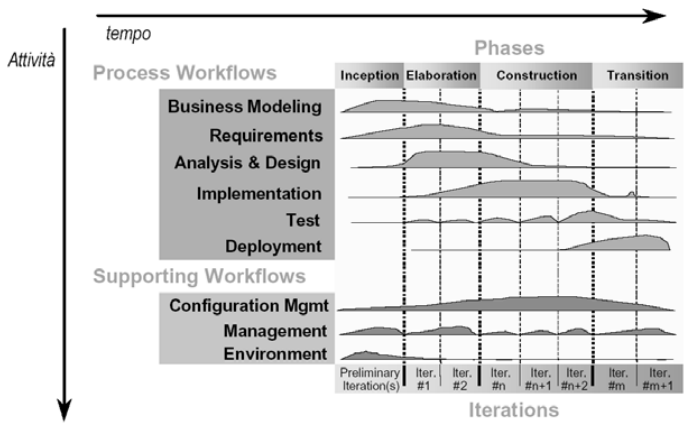
\includegraphics[width= \textwidth]{assets/fasiworkflow}
\end{center}

\section{Pianificazione iterazioni}
\label{sec:pianificazione_iterazioni}
Saranno di seguito elencate le iterazioni svolte durante il progetto, durante lo sviluppo compariranno le iterazioni già effettuate e la pianificazione dell'iterazione successiva.

\begin{center}
	\begin{tabularx}{\tabwidthiter}{ l  X } 
		\toprule
		\multicolumn{2}{c}{\tabtitleiter{Iterazione 01}}  \\
		\cmidrule(l{\cmidrulekern}r{\cmidrulekern}){1-2}
		\tabheaditer{Fase} & Inizio \\ 
		\addlinespace[1em] 
		\tabheaditer{Milestones} & 
		    \begin{enumWork}
			        \item Stesura del documento di richiesta
			        \item Stesura del documento di visione
			        \item Stesura dello studio di fattibilità
			        \item Stesura del contratto
			        \item Inizio stesura del glossario e degli acronimi
			        \item Inizio stesura del documento di pianificazione del progetto
		    \end{enumWork} \\
		\addlinespace[1em]
		\tabheaditer{Stato} &  Effettuata \\
		\bottomrule
	\end{tabularx}
\end{center}

\bigskip

\begin{center}
	\begin{tabularx}{\tabwidthiter}{ l  X } 
		\toprule
		\multicolumn{2}{c}{\tabtitleiter{Iterazione 02}}  \\
		\cmidrule(l{\cmidrulekern}r{\cmidrulekern}){1-2}
		\tabheaditer{Fase} & Elaborazione \\ 
		\addlinespace[1em] 
		\tabheaditer{Milestones} & 
		    \begin{enumWork}
			        \item Stesura del documento di specifica del sistema
			        \item Stesura del documento di specifica dei requisiti
			        \item Stesura del documento dei casi d'uso
			        \item Aggiornamento del glossario e degli acronimi
			        \item Aggiornamento del documento di pianificazione
		    \end{enumWork} \\
		\addlinespace[1em]
		\tabheaditer{Stato} &  In corso \\
		\bottomrule
	\end{tabularx}
\end{center}


\begin{landscape}
\section{Diagramma di Gantt}
\label{sec:diagramma_di_gantt}
Nel seguente diagramma di Gantt sono riportati i periodi di svolgimento di ogni attività effettuata per la realizzazione del sistema.

\begin{center}
	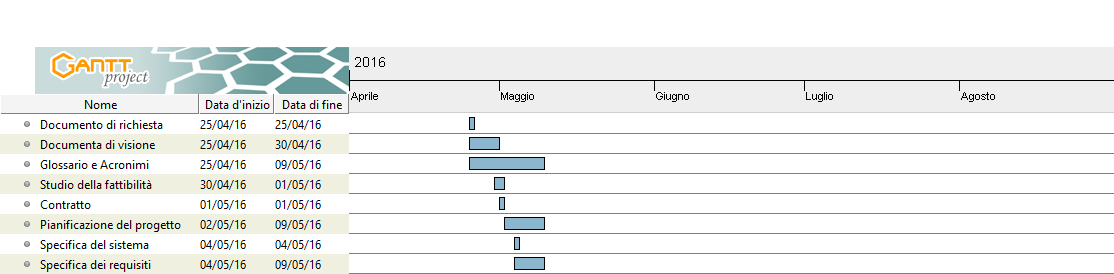
\includegraphics[width=\linewidth]{diagrammaGantt/DiagrammaGantt}
\end{center}
\end{landscape}

\newdate{pianuno}{3}{05}{2016}
\newdate{piandue}{4}{05}{2016}
\section{Revisioni}
\begin{center}
    \begin{tabular}{lll}
        \toprule
        \tabhead{Versione} & \tabhead{Data} & \tabhead{Descrizione} \\
        %   \cmidrule{2-3} 
        \midrule
        1.0 & \displaydate{pianuno} & Prima versione \\
        1.1 & \displaydate{piandue} & Aggiunta iterazione 02 \\
        \bottomrule
    \end{tabular}
\end{center}

    \chapter{Specifica sistema} 
\label{cha:specifica_sistema}

\section{Introduzione} 
In questo documento verrà descritto nel dettaglio il sistema nel suo complesso, in modo più approfondito rispetto al \docref{cha:documento_di_visione}.

\section{Descrizione dettagliata} 
\label{sec:descrizione_dettagliata}
Il portale che si vuole realizzare interagirà con diverse \grupporuolo{figure pubbliche}, che si distinguono tra autenticate e non autenticate. Fra le \grupporuolo{figure pubbliche autenticate} troviamo gli \ruolo{utenti} e i \ruolo{produttori}, mentre i \ruolo{visitatori} sono l'unica \grupporuolo{figura pubblica non autenticata}.
Sono presenti inoltre diverse \grupporuolo{figure amministrative}, quali i \ruolo{redattori}, gli \ruolo{assistenti} e i \ruolo{moderatori}.

\bigskip
\noindent
Le diverse figure presenti si distinguono a seconda di quali funzionalità, messe a disposizione dal sistema, possono utilizzare.

I \ruolo{visitatori} possono effettuare l'iscrizione, diversa a seconda della tipologia di account che si vuole creare, e l'autenticazione. Entrambe possono essere effettuate tramite l'integrazione con i principali Social Network, tuttavia per iscriversi come \ruolo{produttore} tramite Social Network si deve avere un account certificato in esso.

I \ruolo{produttori} hanno a disposizione uno spazio per pubblicizzare i loro prodotti, che da questo momento in avanti chiameremo \emph{vetrina}. Essi potranno dunque personalizzare la loro vetrina, inserendo informazioni e immagini sul \ruolo{produttore}, e possono inserire prodotti o modificare quelli già inseriti. L'inserimento di prodotti seguirà una rigida procedura per garantire la consistenza dei dati e facilitare la ricerca dei prodotti. Potranno inoltre commentare recensioni ai loro prodotti.

Gli \ruolo{utenti} possono valutare oppure effettuare una recensione, la quale aggiunge una descrizione testuale alla valutazione, dei prodotti. Una volta inserita una recensione o una valutazione è possibile modificarla, oppure è possibile eliminare la propria recensione. 
Per permettere di visualizzare velocemente le recensioni più utili, gli \ruolo{utenti} possono dare un giudizio positivo oppure negativo sulle recensioni presenti. Hanno inoltre la possibilità di commentare le recensioni, per permettere una maggiore interazione fra gli \ruolo{utenti}.
Per facilitare l'inserimento di informazioni nel portale sono state inoltre pensate due particolari funzionalità: l'\ruolo{utente} può suggerire un prodotto mancante ad un \ruolo{produttore} iscritto, e tale \ruolo{produttore} potrà scegliere se accettare o rifiutare la richiesta di inserimento, eventualmente modificando le informazioni inserite dall'\ruolo{utente}; inoltre l'\ruolo{utente} potrà suggerire al sistema un prodotto mancante di un \ruolo{produttore} esterno non ancora iscritto al portale. In questo caso il sistema raccoglierà le richieste indirizzate ad uno stesso \ruolo{produttore} e superata una certa soglia si valuterà la possibilità di contattare il \ruolo{produttore} per indurlo ad iscriversi nel portale (per il \ruolo{produttore} sarebbe vantaggioso, in quanto avrebbe molta pubblicità) oppure di creare la sua vetrina in sua vece.
Inoltre gli \ruolo{utenti} possono ricevere consigli sui prodotti che gli potrebbero piacere, tenendo conto dell'esperienza passata nel portale. 

\bigskip
\noindent
Alcune funzionalità sono comuni a diverse figure.

Le \grupporuolo{figure pubbliche autenticate} possono usufruire del sistema di follower/followed, possono quindi seguire altri account per ricevere aggiornamenti da essi, rimuovere account che si stanno seguendo oppure visualizzare gli aggiornamenti dagli account seguiti. Possono inoltre segnalare recensioni/commenti con contenuti non appropriati e aprire tickets per richiedere assistenza.

I \ruolo{visitatori} e gli \ruolo{utenti} possono ricevere consigli sui prodotti simili a quelli che si stanno visualizzando e notizie simili a quelle lette. 

Tutte le \grupporuolo{figure pubbliche} possono effettuare ricerche nel portale, in base a diversi criteri, di prodotti, di notizie e di profili pubblici.
Esse possono inoltre gestire il proprio account, con la possibilità di visualizzare il profilo (pubblico), accedere alle impostazioni (private), effettuare il logout oppure rimuovere l'account. Da notare che l'eventuale rimozione dell'account non comporterà la rimozione dei contenuti inseriti nel portale, ma solo la rimozione dello stesso. Possono inoltre visualizzare i contenuti pubblici del portale, quali le vetrine dei produttori, con eventuali statistiche, i singoli prodotti con le recensioni associate, i profili pubblici altrui con le statistiche associate a quell'account e le notizie presenti nel portale.

\bigskip
\noindent
Segue una descrizione delle funzionalità specifiche delle \grupporuolo{figure amministrative}, le quali oltre ad esse ereditano tutte le funzionalità specifiche degli \ruolo{utenti}.

I \ruolo{redattori} possono aggiungere, modificare o rimuovere notizie provenienti dal dolciario.

Gli \ruolo{assistenti} possono rispondere ai tickets per risolvere i problemi degli \ruolo{utenti}. Hanno inoltre il compito di gestire le iscrizioni dei produttori effettuate direttamente nel portale, controllando la veridicità delle informazioni inserite, ed in caso creare l'account richiesto.

I \ruolo{moderatori} che possono eliminare il contenuto non appropriato, che può essere segnalato tramite apposito ticket, dalle recensioni o dai commenti. Hanno la possibilità di eliminare completamente la recensione o il commento segnalato oppure di modificarle togliendo la parte incriminata. %VALENTINO SE LEGGI QUI DOBBIAMO DECIDERE!!!

\bigskip
\noindent
Nel portale che si vuole realizzare le informazioni sui prodotti sono di fondamentale importanza, perciò elenchiamo di seguito quelle contenute nel sistema:
\begin{itemize}
	\item \infoProdotto{Nome prodotto. }
	\item \infoProdotto{Almeno una foto dell’articolo.}
	\item \infoProdotto{Descrizione di presentazione.}
	\item \infoProdotto{Marca.}
	\item \infoProdotto{Categoria.}
	\item \infoProdotto{Particolarità.}
	\item \infoProdotto{Consistenza.}
	\item \infoProdotto{Ingredienti.}
	\item \infoProdotto{Altri campi} (a seconda di quali ha compilato il \ruolo{produttore}).
\end{itemize}
L'inserimento di queste informazioni è compito del \ruolo{produttore}, il quale seguirà una rigida procedura che sarà descritta nel dettaglio durante la specifica delle funzionalità.


\newdate{sisuno}{04}{05}{2016}
\section{Revisioni}
\begin{center}
    \begin{tabular}{lll}
        \toprule
        	\tabhead{Versione} & \tabhead{Data} & \tabhead{Descrizione} \\
		\cmidrule(l{\cmidrulekern}r{\cmidrulekern}){1-3}
        	1.0 & \displaydate{sisuno} & Prima versione \\
        \bottomrule
    \end{tabular}
\end{center}

    \chapter{Specifica requisiti} 
\label{cha:specifica_requisiti}

\section{Introduzione} 
In questo documento sono specificati nel dettaglio tutti i requisiti del sistema, suddivisi in funzionali e non funzionali.
Per organizzare in modo corretto le informazioni è stato adottato un sistema di codifica dei requisiti, descritto nella prossima sezione.

\section{Struttura del documento}
\label{sec:struttura_del_documento}

I requisiti mostrati sono prima elencati, per una più facile consultazione, e in seguito sono descritti in apposite tabelle. 
Ogni tabella contiene diverse informazioni:
\begin{itemize}
	\item Un \campiTabReq{id} per identificare univocamente il requisito.
	\item Un \campiTabReq{titolo} per semplificare il riconoscimento del requisito.
	\item Una \campiTabReq{descrizione} per indicare in cosa consiste la funzionalità rappresentata dal requisito.
	\item Un \campiTabReq{tipo} per indicare se il requisito è funzionale o non funzionale
	\item Una \campiTabReq{priorità} per indicare il grado di importanza del requisito.
	\item Lo \campiTabReq{stato} per indicare l'idoneità del requisito.
\end{itemize}

\subsection{Identificativo dei requisiti}
\label{subsec:identificativo_dei_requisiti}

Di seguito è spiegato come interpretare l'identificativo dei requisiti.
Un identificativo è della forma:
\begin{center}
	\subsubreq{tipo}{contesto}{categoria}{req}{[sottoreq]}{[\dots]}
\end{center}

\noindent
Segue una descrizione di ogni campo utilizzato nell'identificatore:
\begin{itemize}
	\item Il \campiIdReq{tipo} può essere:
	\begin{descriptionInd}
		\item[RF] indica un requisito funzionale.
		\item[RNF] indica un requisito non funzionale.
	\end{descriptionInd}

	\item Il \campiIdReq{contesto} serve ad identificare a quali figure è rivolta una data funzionalità, è un numero composto da 6 cifre ognuna delle quali può assumere un valore 0 oppure 1. La posizione della cifra si riferisce ad una specifica figura, se la cifra i-esima vale 1 significa che l'i-esima figura è presente nel contesto del requisitio, altrimenti no.
	Di seguito elenchiamo ogni posizione a quale figura riferisce: 
	\begin{descriptionInd}
		\item[1\textdegree\ bit] Visitatore.
		\item[2\textdegree\ bit] Utente.
		\item[3\textdegree\ bit] Produttore.
		\item[4\textdegree\ bit] Redattore.
		\item[5\textdegree\ bit] Assistente.
		\item[6\textdegree\ bit] Moderatore.
	\end{descriptionInd}		

	\item La \campiIdReq{categoria} è una lettera utilizzata per raggruppare i requisiti con scopi simili.
	Le categorie per i requisiti funzionali sono le seguenti:
	\begin{descriptionInd}
		\item[A] Iscrizione e autenticazione.
		\item[B] Gestione iscrizione.
		\item[C] Gestione vetrina.
		\item[D] Ricerca.
		\item[E] Gestione recensioni.
		\item[F] Gestione notizie.
		\item[G] Gestione follower/followed.
		\item[H] Gestioni suggerimenti.
		\item[I] Gestione account.
		\item[L] Visualizzazione contenuti.
	\end{descriptionInd}	
	Le categorie per i requisiti non funzionali sono le seguenti:
	\begin{descriptionInd}
		\item[A] Sicurezza.
		\item[B] Portabilità.
		\item[C] Usabilità.
		\item[D] Implementazione.
	\end{descriptionInd}	

	\item Il campo \campiIdReq{req} è un numero progressivo utilizzato per identificare in modo univoco un requisito all'interno della sua categoria.

	\item Il campo \campiIdReq{sottoreq} (opzionale) è un numero progressivo utilizzato per identificare in modo univoco un sotto--requisito di un dato requisito. Ci possono essere diversi campi sottoreq consecutivi, per esplicitare una nidificazione dei requisiti più dettagliata.
\end{itemize}

\subsection{Priorità}
\label{subsec:priorita}

La priorità di un requisito identifica quanto un requisito sia importante ai fini del completamento del sistema.
Qui di seguito sono elencati in breve i ``gradi di giudizio'' della priorità di un requisito:

\begin{descriptionInd}
	\item[Priorità Alta] Requisiti che il sistema deve necessariamente soddisfare.
	\item[Priorità Media] Requisiti la cui assenza non comporta grossi problemi per la soddisfacibilità del progetto: i requisiti base riescono comunque ad essere soddisfatti, con qualche sacrificio in termini di funzionalità. 
	\item[Priorità Bassa] Requisiti la cui assenza non comporta alcun tipo di problema per la soddisfacibilità del progetto. Questi requisiti possono anche visti come superflui o non strettamente necessari. La loro inclusione comporta un miglioramento della qualità complessiva dell’offerta dei servizi e delle funzionalità del progetto.
\end{descriptionInd}

\section{Elenco dei requisiti}
\label{sec:elenco_dei_requisiti}
Di seguito sono elencati tutti i requisiti, suddivisi in funzionali e non funzionali.

\subsection{Requisiti funzionali}
Vengono di seguito elencati i requisiti funzionali:
%USAGE: {keyrequisito}{\ereq{tipo}{contesto}{categoria}}{titolo} - doublelink automatico con \refDef{keyrequisito}
\begin{itemize} 
	\item \reqItem{req:iscrizione}{\ereq{RF}{100000}{A}}{Iscrizione}
	\item \reqItem{req:iscrizionePortale}{\esubreq{RF}{100000}{A}}{Iscrizione tramite modulo del portale}
	\item \reqItem{req:iscrizioneSocial}{\esubreq{RF}{100000}{A}}{Iscrizione tramite Social Network}
	\item \reqItem{req:iscrizioneSocialVer}{\esubsubreq{RF}{100000}{A}}{Iscrizione tramite Social Network verificati}
	\item \reqItem{req:iscrizioneSocialNotVer}{\esubsubreq{RF}{100000}{A}}{Iscrizione tramite Social Network non verificati}
	\item \reqItem{req:iscrizioneApprovazione}{\esubreq{RF}{100000}{A}}{Iscrizione tramite approvazione}
	
	\item \reqItem{req:login}{\ereq{RF}{100000}{A}}{Login}
	\countReset 
	
	\item \reqItem{req:approvazioneIscrizione}{\ereq{RF}{000010}{B}}{Approvazione iscrizione}
	
	\item \reqItem{req:rimozioneAccountAltrui}{\ereq{RF}{000001}{B}}{Rimozione account altrui}
	\countReset
	
	\item \reqItem{req:personalizzaVetrina}{\ereq{RF}{001000}{C}}{Personalizzione vetrina}
	\item \reqItem{req:personalizzaVetrinaInsDesc}{\esubreq{RF}{001000}{C}}{Inserimento descrizione}
	\item \reqItem{req:personalizzaVetrinaInsImg}{\esubreq{RF}{001000}{C}}{Inserimento immagine}
	\item \reqItem{req:personalizzaVetrinaInsProd}{\esubreq{RF}{001000}{C}}{Inserimento prodotto}
	\item \reqItem{req:personalizzaVetrinaModProd}{\esubreq{RF}{001000}{C}}{Modifica prodotto}
	
	\item \reqItem{req:statistichePrivateVetrina}{\ereq{RF}{001000}{C}}{Visualizzazione statistiche private della vetrina}
	\countReset
	
	\item \reqItem{req:ricercaInfo}{\ereq{RF}{111111}{D}}{Ricerca informazioni}
	\item \reqItem{req:ricercaProdotto}{\esubreq{RF}{111111}{D}}{Ricerca prodotto}
	\item \reqItem{req:ricercaProfilo}{\esubreq{RF}{111111}{D}}{Ricerca profilo}
	\item \reqItem{req:ricercaNotizia}{\esubreq{RF}{111111}{D}}{Ricerca notizia}

	\item \reqItem{req:richiestaInsProdotto}{\ereq{RF}{010000}{D}}{Richiesta inserimento prodotto a un produttore iscritto}

	\item \reqItem{req:richiestaInsProduttore}{\ereq{RF}{010000}{D}}{Richiesta inserimento prodotto e del suo produttore}
	\countReset

	\item \reqItem{req:valutazioneProdotto}{\ereq{RF}{010111}{E}}{Valutazione prodotto}
	\item \reqItem{req:inserisciValutazioneProdotto}{\esubreq{RF}{010111}{E}}{Inserimento valutazione}
	\item \reqItem{req:modificaValutazioneProdotto}{\esubreq{RF}{010111}{E}}{Modifica valutazione inserita}
	\item \reqItem{req:eliminaValutazioneProdotto}{\esubreq{RF}{010111}{E}}{Rimozione valutazione inserita}

	\item \reqItem{req:recensioneProdotto}{\ereq{RF}{010111}{E}}{Recensione prodotto}
	\item \reqItem{req:inserisciRecensioneProdotto}{\esubreq{RF}{010111}{E}}{Inserimento recensione}
	\item \reqItem{req:modificaRecensioneProdotto}{\esubreq{RF}{010111}{E}}{Modifica valutazione inserita}
	\item \reqItem{req:eliminaRecensioneProdotto}{\esubreq{RF}{010111}{E}}{Rimozione recensione inserita}

	\item \reqItem{req:commentoRecensione}{\ereq{RF}{011111}{E}}{Commento a recensione}
	
	\item \reqItem{req:valutaRecensione}{\ereq{RF}{010111}{E}}{Valutazione recensione}
	
	\item \reqItem{req:segnalazioneContenuti}{\ereq{RF}{011111}{E}}{Segnalazione contenuti inappropriati}
	
	\item \reqItem{req:rimozioneRecensioneInap}{\ereq{RF}{000001}{E}}{Rimozione recensione inappropriata}
	\countReset

	\item \reqItem{req:inserimentoNotizia}{\ereq{RF}{000100}{F}}{Inserimento notizia}
	
	\item \reqItem{req:modificaNotizia}{\ereq{RF}{000100}{F}}{Modifica notizia}
	
	\item \reqItem{req:rimozioneNotizia}{\ereq{RF}{000100}{F}}{Rimozione notizia}
	\countReset
	
	\item \reqItem{req:followAccount}{\ereq{RF}{011111}{G}}{Follow account}
	
	\item \reqItem{req:unFollowAccount}{\ereq{RF}{011111}{G}}{Unfollow account}
	\countReset

	\item \reqItem{req:suggerimentoProdotti}{\ereq{RF}{011111}{H}}{Suggerimento prodotti intelligente}
	
	\item \reqItem{req:prodottiSimili}{\ereq{RF}{011111}{H}}{Suggerimento prodotti simili}

	\item \reqItem{req:notizieSimili}{\ereq{RF}{011111}{H}}{Suggerimento notizie simili}
	\countReset

	\item \reqItem{req:accessoProfilo}{\ereq{RF}{011111}{I}}{Accesso al proprio profilo}
	
	\item \reqItem{req:accessoImpostazioni}{\ereq{RF}{011111}{I}}{Accesso alle proprie impostazioni}

	\item \reqItem{req:rimozioneAccountProprio}{\ereq{RF}{011111}{I}}{Rimozione account proprio}
	
	\item \reqItem{req:logout}{\ereq{RF}{011111}{I}}{Logout}
	\countReset
	
	\item \reqItem{req:visualizzazioneVetrina}{\ereq{RF}{111111}{L}}{Visualizzazione vetrina}
	\item \reqItem{req:visualizzazioneStatistichePubVetrina}{\esubreq{RF}{111111}{L}}{Visualizzazione statische pubbliche vetrina}
	\item \reqItem{req:visualizzazioneProdottiVetrina}{\esubreq{RF}{111111}{L}}{Visualizzazione prodotti esposti in vetrina}

	\item \reqItem{req:visualizzazioneProdotto}{\ereq{RF}{111111}{L}}{Visualizzazione prodotto}
	\item \reqItem{req:visualizzazioneInfoProdotto}{\esubreq{RF}{111111}{L}}{Visualizzazione informazioni del prodotto}
	\item \reqItem{req:visualizzazioneRecProdotto}{\esubreq{RF}{111111}{L}}{Visualizzazione recensioni associate al prodotto}
	\item \reqItem{req:visualizzazioneStatProdotto}{\esubreq{RF}{111111}{L}}{Visualizzazione statistiche del prodotto}

	\item \reqItem{req:visualizzazioneProfilo}{\ereq{RF}{111111}{L}}{Visualizzazione profilo pubblico}
	\item \reqItem{req:visualizzazioneInfoProfilo}{\esubreq{RF}{111111}{L}}{Visualizzazione informazioni di un profilo pubblico}
	\item \reqItem{req:visualizzazioneStatProfilo}{\esubreq{RF}{111111}{L}}{Visualizzazione statistiche di un profilo pubblico}

	\item \reqItem{req:visualizzazioneNotizie}{\ereq{RF}{111111}{L}}{Visualizzazione notizie}
	
	\item \reqItem{req:visualizzazioneAggF}{\ereq{RF}{011111}{L}}{Visualizzazione aggiornamenti dai followed}
\end{itemize}	


\subsection{Requisiti non funzionali}
\label{sub:requisiti_non_funzionali}


\section{Descrizione dei requisiti}
\label{sec:descrizione_dei_requisiti}
Di seguito sono presenti tutte le descrizioni dei requisiti, suddivise in funzionali e non funzionali.

\subsection{Requisiti funzionali}
Vengono di seguito riportate le tabelle che descrivono nel dettaglio ogni requisito funzionale.

\reqTabRF{req:iscrizione}{}{}{}

\tabreqvspace

\reqTabRF{req:iscrizionePortale}{}{}{}

\tabreqvspace

\reqTabRF{req:iscrizioneSocial}{}{}{}

\tabreqvspace

\reqTabRF{req:iscrizioneSocialVer}{}{}{}

\tabreqvspace

\reqTabRF{req:iscrizioneSocialNotVer}{}{}{}

\tabreqvspace

\reqTabRF{req:iscrizioneApprovazione}{}{}{}

\tabreqvspace

\reqTabRF{req:login}{}{}{}

\tabreqvspace

\reqTabRF{req:approvazioneIscrizione}{}{}{}

\tabreqvspace

\reqTabRF{req:rimozioneAccountAltrui}{}{}{}

\tabreqvspace

\reqTabRF{req:personalizzaVetrina}{}{}{}

\tabreqvspace

\reqTabRF{req:personalizzaVetrinaInsDesc}{}{}{}

\tabreqvspace

\reqTabRF{req:personalizzaVetrinaInsImg}{}{}{}

\tabreqvspace

\reqTabRF{req:personalizzaVetrinaInsProd}{}{}{}

\tabreqvspace

\reqTabRF{req:personalizzaVetrinaModProd}{}{}{}

\tabreqvspace

\reqTabRF{req:statistichePrivateVetrina}{}{}{}

\tabreqvspace

\reqTabRF{req:ricercaInfo}{}{}{}

\tabreqvspace

\reqTabRF{req:ricercaProdotto}{}{}{}

\tabreqvspace

\reqTabRF{req:ricercaProfilo}{}{}{}

\tabreqvspace

\reqTabRF{req:ricercaNotizia}{}{}{}

\tabreqvspace

\reqTabRF{req:richiestaInsProdotto}{}{}{}

\tabreqvspace

\reqTabRF{req:richiestaInsProduttore}{}{}{}

\tabreqvspace

\reqTabRF{req:valutazioneProdotto}{}{}{}

\tabreqvspace

\reqTabRF{req:inserisciValutazioneProdotto}{}{}{}

\tabreqvspace

\reqTabRF{req:modificaValutazioneProdotto}{}{}{}

\tabreqvspace

\reqTabRF{req:eliminaValutazioneProdotto}{}{}{}

\tabreqvspace

\reqTabRF{req:recensioneProdotto}{}{}{}

\tabreqvspace

\reqTabRF{req:inserisciRecensioneProdotto}{}{}{}

\tabreqvspace

\reqTabRF{req:modificaRecensioneProdotto}{}{}{}

\tabreqvspace

\reqTabRF{req:eliminaRecensioneProdotto}{}{}{}

\tabreqvspace

\reqTabRF{req:commentoRecensione}{}{}{}

\tabreqvspace

\reqTabRF{req:valutaRecensione}{}{}{}

\tabreqvspace

\reqTabRF{req:segnalazioneContenuti}{}{}{}

\tabreqvspace

\reqTabRF{req:rimozioneRecensioneInap}{}{}{}

\tabreqvspace

\reqTabRF{req:inserimentoNotizia}{}{}{}

\tabreqvspace

\reqTabRF{req:modificaNotizia}{}{}{}

\tabreqvspace

\reqTabRF{req:rimozioneNotizia}{}{}{}

\tabreqvspace

\reqTabRF{req:followAccount}{}{}{}

\tabreqvspace

\reqTabRF{req:unFollowAccount}{}{}{}

\tabreqvspace

\reqTabRF{req:suggerimentoProdotti}{}{}{}

\tabreqvspace

\reqTabRF{req:prodottiSimili}{}{}{}

\tabreqvspace

\reqTabRF{req:notizieSimili}{}{}{}

\tabreqvspace

\reqTabRF{req:accessoProfilo}{}{}{}

\tabreqvspace

\reqTabRF{req:accessoImpostazioni}{}{}{}

\tabreqvspace

\reqTabRF{req:rimozioneAccountProprio}{}{}{}

\tabreqvspace

\reqTabRF{req:logout}{}{}{}

\tabreqvspace

\reqTabRF{req:visualizzazioneVetrina}{}{}{}

\tabreqvspace

\reqTabRF{req:visualizzazioneStatistichePubVetrina}{}{}{}

\tabreqvspace

\reqTabRF{req:visualizzazioneProdottiVetrina}{}{}{}

\tabreqvspace

\reqTabRF{req:visualizzazioneProdotto}{}{}{}

\tabreqvspace

\reqTabRF{req:visualizzazioneInfoProdotto}{}{}{}

\tabreqvspace

\reqTabRF{req:visualizzazioneRecProdotto}{}{}{}

\tabreqvspace

\reqTabRF{req:visualizzazioneStatProdotto}{}{}{}

\tabreqvspace

\reqTabRF{req:visualizzazioneProfilo}{}{}{}

\tabreqvspace

\reqTabRF{req:visualizzazioneInfoProfilo}{}{}{}

\tabreqvspace

\reqTabRF{req:visualizzazioneStatProfilo}{}{}{}

\tabreqvspace

\reqTabRF{req:visualizzazioneNotizie}{}{}{}

\tabreqvspace

\reqTabRF{req:visualizzazioneAggF}{}{}{}

\subsection{Requisiti non funzionali}
Vengono di seguito riportate le tabelle che descrivono nel dettaglio ogni requisito non funzionale.

    %%Date versioni
%Versione 1
\newdate{versioneuno}{22}{04}{2016}
\chapter{Proposta di progetto} 

\section{Introduzione}
L’associazione italiana amatori di cioccolato\footnote{Raggiungibile al seguente indirizzo: \url{http://www.chococlub.com/}} è intenzionata a lanciare un nuovo portale.
Le richieste per questo sistema sono le seguenti:
\begin{itemize}
	\item possibilità da parte dei produttori di inserire (o modificare, o rimuovere) i propri prodotti (sia cioccolato che dolci a base di esso) nel catalogo generale.
	\item ricerca sul catalogo dei prodotti, anche avanzata, sulla base delle caratteristiche degli stessi.
	\item sezione notizie.
	\item funzionalità stile social (recensioni di prodotti e sistema di follower/follo\-wed).
\end{itemize}
Volontà dell'associazione è ottenere un sistema di facile consultazione e aggiornamento.
Esso dovrà permettere agli utenti del servizio di ricercare e recensire prodotti come pure di consigliarne altri.
L'interazione tra utenti invece, è richiesta tramite un sistema di follower/followed che faccia da contorno al sistema principale, quindi non invasivo, ma che permetta ai fruitori del servizio (i follower) di ottenere informazioni riguardo attività da parte di chi seguono (i followed).
Nel sistema follower/followed chiunque può essere un follower (sia gli utenti semplici, sia i produttori) nonché followed.

È stato deciso di non utilizzare i contenuti attualmente presenti sul sito dell’associazione, per le seguenti motivazioni: il sito è statico e di difficile consultazione e analisi, oltretutto la maggior parte dei contenuti non è aggiornata. Inoltre, i dati attualmente contenuti non riguardano principalmente i prodotti, ma le pasticcerie come attività commerciali, quindi non sono utili per gli obiettivi del nuovo portale.
 
Per questo motivo è stato deciso di realizzare un portale ex novo, avvalendosi dell’utilizzo di un \gls{cms}.

Dopo un’attenta analisi della richiesta ed uno studio del settore, abbiamo elaborato la seguente proposta di realizzazione della piattaforma. Va fatto notare che il punto di forza del servizio saranno le informazioni sui prodotti esclusivamente di cioccolata, ma è stato deciso di includere anche la catalogazione di dolci che la contengono, per rivolgersi ad una più ampia fetta di mercato.

\section{Descrizione generale}
Come da richiesta, il portale permetterà agli utenti di reperire informazioni ad alta affidabilità riguardo la cioccolata ed i suoi produttori.
Tali informazioni copriranno ogni aspetto riguardante il prodotto, visto che saranno anche arricchite dagli utenti attraverso un sistema di recensioni e commenti, così da rendere completa la descrizione dei prodotti (includendo l'opinione dell'utente stesso).
Per i produttori, il portale sarà un mezzo di pubblicità in quanto avranno una vetrina personalizzata per esporre i propri prodotti e saranno essi stessi ad inserire tutte le specifiche dei loro prodotti, ovvero le informazioni che gli utenti potranno reperire.
Il portale avrà diversi tipi di ruoli amministrativi e di utenze; segue una breve descrizione delle stesse, in seguito approfondita. 
Le \ruolo{Utenze}:
\begin{descriptionInd}
	\item[Produttore] si potrà iscrivere al portale solo tramite account verificati da siti terzi o tramite approvazione privata, contattando direttamente il supporto. Avrà il compito di creare e mantenere aggiornata la sua vetrina. Sarà a lui delegata l’aggiunta di ogni suo prodotto, anche in seguito a richieste da parte degli utenti.
	
	\item[Utente] si potrà iscrivere al portale, anche tramite account di siti terzi. La loro funzionalità principale, oltre la ricerca dei prodotti, sarà la possibilità di recensire e/o valutare i prodotti stessi. 
\end{descriptionInd}
Le \ruolo{Figure di gestione del portale}:
\begin{descriptionInd}
	\item[Web Admin] avrà accesso completo al pannello di controllo del \gls{cms}
	
	\item[Newser] avrà, oltre alle funzionalità base dell’utente, il compito di gestire gli articoli e le notizie dal mondo dolciario.
	
	\item[Support] gestirà l’e-mail del portale rispondendo alle richieste di supporto e avrà il compito di approvare le richieste di iscrizione da parte dei produttori (tali richieste saranno inviate tramite form per una più facile gestione di esse).
	
	\item[Moderatore] avrà il compito di gestire segnalazioni di utenti eliminando/modificando eventuali contenuti non consoni presenti in recensioni.
\end{descriptionInd}

\noindent
Alcune funzionalità che potranno essere implementate in futuro sono: 
\begin{itemize}
	\item l’implementazione della \funfutura{wishlist} per ricordarsi dei prodotti che si vorrebbero provare.

	\item l’aggiunta del \funfutura{produttore delegato}, una figura necessaria per aiutare le piccole realtà dolciarie che si occuperà di gestire le vetrine al loro posto.

	\item Aggiunta dei commenti alle \funfutura{notizie}.
\end{itemize}

Per la fase iniziale di riempimento del portale, sarà compito di ChocoClub stessa prendere contatti con le molte pasticcerie artigianali già affiliate e le case produttrici, affinché esse si iscrivano al portale, per avere un buon numero di contenuti di partenza. 

\section{Descrizione funzionalità principali}
Di seguito è presente una panoramica generale di alcune delle principali funzionalità che saranno presenti nel portale, tale elenco potrà essere soggetto a modifiche nel corso dello sviluppo.
\begin{enumerate}
	\item \bloccofun{Iscrizione \& Autenticazione} \label{bloccofun:iscAut}
		\begin{enumerate}        	
			\item	\begin{descriptionNext}
						\item[Iscrizione tramite portale] Permette l’iscrizione direttamente tramite il portale. 
					\end{descriptionNext} \label{fun:isc.portale}
						                      
			\item 	\begin{descriptionNext}
						\item[Iscrizione tramite account terzi verificati] Si tratta della possibilità di iscriversi tramite account di altri servizi come LinkedIn, Facebook e Twitter, purché risultino “verificati” anche su quelle piattaforme.							
					\end{descriptionNext} \label{fun:isc.terziv}
					                       
			\item 	\begin{descriptionNext}
						\item[Iscrizione tramite account terzi non verificati]	È possibile utilizzare un account di siti terzi Google o Facebook per iscriversi							 
					\end{descriptionNext} \label{fun:isc.terzinv}
					                       
			\item 	\begin{descriptionNext}
						\item[Iscrizione tramite approvazione] Si tratta della possibilità per i produttori di iscriversi in modo verificato al portale, senza possedere un account già verificato su siti terzi.
						               
					\end{descriptionNext} \label{fun:isc.appr}
					                       
			\item 	\begin{descriptionNext}
						\item[Login] Permette di fare il login nel sistema utilizzando le credenziali con cui ci si è registrati.							
					\end{descriptionNext} \label{fun:aut.login}			
		\end{enumerate}
		
	\item \bloccofun{Gestione iscrizione}	\label{bloccofun:gestisc}		
		\begin{enumerate}        
			\item	\begin{descriptionNext}
						\item[Approvazione iscrizione] Si tratta della funzione relativa alla \funref{fun:isc.appr}, permette di approvare le richieste di iscrizione.
					\end{descriptionNext}	\label{fun:appr.iscr}
					                      
			\item	\begin{descriptionNext}
						\item[Rimozione account altrui] Permette di eliminare un account, ma NON le recensioni e valutazioni ad esso correlate nel caso di utenti e NON rimuove i prodotti nel caso di account produttore.
					\end{descriptionNext}	\label{fun:rim.iscr}
		\end{enumerate}
		
	\item \bloccofun{Gestione spazio dedicato alla presentazione prodotti (vetrina)}	\label{bloccofun:gestvet}		
		\begin{enumerate}        
			\item	\begin{descriptionNext}
						\item[Inserimento descrizione e immagine vetrina] Permette di avere a disposizione una vetrina pubblica, in cui ci sarà la descrizione del produttore e in cui verranno presentati i suoi prodotti. La funzionalità permette di personalizzare la vetrina attraverso un campo testuale (descrizione) ed un’immagine di sfondo.
					\end{descriptionNext}	\label{fun:ins.vetr}
					                      
			\item	\begin{descriptionNext}
						\item[Inserimento prodotto in vetrina] Permette l’aggiunta di un prodotto alla vetrina. Questa funzionalità segue un rigido protocollo per far sì che le informazioni inserite siano complete e coerenti. 
						Durante l’inserimento di un prodotto è necessario immettere: il \campo{nome del prodotto} con una sua \campo{descrizione} ed almeno una \campo{foto}. 
						È inoltre necessario compilare un modulo che contiene campi a \dominiocampo{scelta multipla} e campi con \dominiocampo{tag dinamici}, di cui a seguire una breve descrizione: il sistema metterà a disposizione una grande lista dei possibili tag, che saranno suggeriti come auto-completamento all’utilizzatore durante la compilazione del campo correlato.
						L’utilizzo di un tag non in lista è permesso, ma esso verrà sottoposto ad una fase di verifica che se superata comporterà l’aggiunta in lista, in caso contrario verrà rimosso anche dal prodotto. Sarà specificato un limite massimo e minimo di tag da inserire per prodotto.
						Nel modulo verrà chiesta la \campo{marca} (a scelta fra quelle associate al produttore che sta inserendo il prodotto), la \campo{categoria} del prodotto che si sta inserendo (a scelta fra \dominiocampo{Dolce al cioccolato} oppure \dominiocampo{cioccolato}), \campo{particolarità} (risposta con \dominiocampo{tag dinamici}),  la \campo{consistenza} (a scelta fra \dominiocampo{solida}, \dominiocampo{liquida} oppure \dominiocampo{spalmabile}), gli \campo{ingredienti} (risposta con \dominiocampo{tag dinamici}).
						Durante la compilazione del modulo di un prodotto è possibile compilare ulteriori campi (oltre a quelli proposti di default) scegliendo fra quelli messi a disposizione dal sistema, per migliorare la descrizione del prodotto e facilitarne la ricerca.
					\end{descriptionNext}	\label{fun:ins.prod}

			\item	\begin{descriptionNext}
						\item[Modifica prodotto in vetrina] Permette la modifica delle caratteristiche dei prodotti presenti, secondo gli stessi campi della \funref{fun:ins.prod}. Permette, inoltre, di etichettare un prodotto come fuori produzione.
					\end{descriptionNext} \label{fun:mod.login}

			\item	\begin{descriptionNext}
						\item[Visualizzazione statistiche vetrina privata] Mostra statistiche della vetrina, in rapporto al tempo; riassume le recensioni dei prodotti in essa presenti, in modo filtrabile e ordinabile in base a diversi criteri e permette di visualizzare il numero di visite ricevute.
					\end{descriptionNext} \label{fun:vis.vetrPr}	 	  				
		\end{enumerate}			
		
	\item \bloccofun{Ricerca} \label{bloccofun:ric}
		\begin{enumerate}
			\item	\begin{descriptionNext}
						\item[Ricerca prodotti tramite diversi criteri] Permette di effettuare ricerche, le ricerche potranno basarsi su qualsiasi campo della scheda del prodotto e dettagli del produttore. Sarà possibile ordinare i risultati.
					\end{descriptionNext}	\label{fun:ric.prod}

			\item	\begin{descriptionNext}
						\item[Ricerca profili pubblici] Permette di ricercare e in seguito visualizzare tramite l’apposita funzionalità, i profili pubblici di utenti e/o produttori.
					\end{descriptionNext}	\label{fun:ric.prof}

			\item	\begin{descriptionNext}
						\item[Ricerca notizie] Permette di effettuare ricerche sulle notizie pubblicate nel portale.
					\end{descriptionNext}	\label{fun:ric.not}
		\end{enumerate}

	\item \bloccofun{Gestione recensioni} \label{bloccofun:gestrec}
		\begin{enumerate}
			\item	\begin{descriptionNext}
						\item[Valutazione prodotto] Permette di esprimere una valutazione su scala limitata di un prodotto.
					\end{descriptionNext}	\label{fun:val.prod}

			\item	\begin{descriptionNext}
						\item[Recensione prodotto esistente] Permette di aggiungere, alla semplice \funref{fun:val.prod}, anche una descrizione testuale della recensione, più completa.
					\end{descriptionNext}	\label{fun:rece.prod}

			\item	\begin{descriptionNext}
						\item[Richiesta inserimento di un prodotto a un produttore]Permette di segnalare ad un produttore la mancanza di un suo prodotto tra quelli presenti nel sistema.
					\end{descriptionNext}	\label{fun:ric.prodotto}

			\item	\begin{descriptionNext}
						\item[Richiesta inserimento di un prodotto e del suo produttore]Permette di segnalare al personale incaricato l’assenza di un produttore ed allo stesso tempo di uno suo specifico prodotto.
					\end{descriptionNext}	\label{fun:ric.produttore}

			\item	\begin{descriptionNext}
						\item[Modifica recensione propria] Permette di modificare il campo testuale menzionato nella \funref{fun:rece.prod} della propria recensione.
					\end{descriptionNext}		\label{fun:mod.recPropria}

			\item	\begin{descriptionNext}
						\item[Modifica recensione altrui] Permette di modificare il campo testuale menzionato nella  \funref{fun:rece.prod} di una qualsiasi recensione.
					\end{descriptionNext}		\label{fun:mod.recAltrui}

			\item	\begin{descriptionNext}
						\item[Modifica valutazione] Permette di modificare la valutazione sia per recensioni che per semplici valutazioni.
					\end{descriptionNext}		\label{fun:mod.valPropia}

			\item	\begin{descriptionNext}
						\item[Valutazione recensione] Permette di esprimere una valutazione positiva o negativa sulle recensioni. Ciò permetterà di stabilire quali recensioni sono più utili.
					\end{descriptionNext}		\label{fun:val.rec}

			\item	\begin{descriptionNext}
						\item[Elimina recensione propria] Permette di eliminare la propria recensione. 
					\end{descriptionNext}		\label{fun:del.recPropia}

			\item	\begin{descriptionNext}
						\item[Elimina recensione altrui] Permette di eliminare una qualsiasi recensione.
					\end{descriptionNext}	 \label{fun:del.recAltrui}
					
			\item	\begin{descriptionNext}
						\item[Commento a recensione] Permette di commentare una qualsiasi recensione.
					\end{descriptionNext}	\label{fun:comm.rec}

			\item	\begin{descriptionNext}
						\item[Segnalazione contenuti] Permette di segnalare contenuti come recensioni e commenti alle stesse, se non consoni (secondo il regolamento del servizio). 
					\end{descriptionNext}	\label{fun:report.cont}
		\end{enumerate}

	\item \bloccofun{Gestione notizie} \label{bloccofun:gestnot}
		\begin{enumerate}
			\item	\begin{descriptionNext}
						\item[Consultazione notizie] Permette la visualizzazione delle notizie inserite nel portale, in base a preferenze dell’utente e impostazioni del gestore.
					\end{descriptionNext}	\label{fun:vis.not}

			\item	\begin{descriptionNext}
						\item[Inserisci notizia] Permette di aggiungere una notizia visibile tramite la \funref{fun:vis.not}.
					\end{descriptionNext}	\label{fun:ins.not}
					
			\item	\begin{descriptionNext}
						\item[Modifica notizia] Permette di modificare una notizia già esistente.
					\end{descriptionNext}	 \label{fun:mod.not}

			\item	\begin{descriptionNext}
						\item[Elimina notizia] Permette di eliminare una notizia già esistente.
					\end{descriptionNext}	\label{fun:del.not}
		\end{enumerate}

	\item \bloccofun{Gestione follower/followed} \label{bloccofun:gestfoll}
		\begin{enumerate}
			\item	\begin{descriptionNext}
						\item[Visualizzazione aggiornamenti followed] Mostra gli aggiornamenti e le notizie relativi ai propri followed.
						Questo sistema permetterà di ottenere una vista sulle attività dei followed, ovvero: nuova recensione, nuovo followed, nuova valutazione se si tratta di un utente; nuovo prodotto, prodotto fuori produzione se invece di tratta di un produttore.
					\end{descriptionNext}	\label{fun:vis.foll}

			\item	\begin{descriptionNext}
						\item[Follow account] Permette di seguire un account e ricevere da esso notizie e aggiornamenti. 
					\end{descriptionNext}	\label{fun:foll.acc}
					
			\item	\begin{descriptionNext}
						\item[Unfollow account] Permette di non seguire più un account che si segue. 
					\end{descriptionNext} \label{fun:unfoll.acc}
		\end{enumerate}

	\item \bloccofun{Gestioni suggerimenti} \label{bloccofun:gestsugg}
		\begin{enumerate}
			\item	\begin{descriptionNext}
						\item[Ti potrebbero piacere\dots] La funzionalità permette di ottenere suggerimenti ad hoc, essi potranno essere basati su diversi parametri: affinità con prodotti per i quali ha già espresso preferenza, informazioni presenti nel profilo (come il luogo di residenza per prodotti artigianali) e recensioni di utenti seguiti.
					\end{descriptionNext}	\label{fun:cons.prod}

			\item	\begin{descriptionNext}
						\item[Prodotti simili a\dots] Permette di suggerire prodotti simili a quello che si sta visualizzando sulla base di diversi criteri.
					\end{descriptionNext}	\label{fun:prod.sim}
					
			\item	\begin{descriptionNext}
						\item[Notizie simili a\dots] Permette di suggerire articoli e notizie sulla base dell’articolo che si sta attualmente leggendo.
					\end{descriptionNext}	\label{fun:not.sim}
		\end{enumerate}

	\item \bloccofun{Gestione account} \label{bloccofun:gestacc}
		\begin{enumerate}
			\item	\begin{descriptionNext}
						\item[Visualizzazione profilo] Permette di visualizzare il proprio profilo.
					\end{descriptionNext}	\label{fun:vis.prof}

			\item	\begin{descriptionNext}
						\item[Accesso alle impostazioni] Permette di accedere alle impostazioni dell’account. Le impostazioni variano a seconda del tipo di account. Per gli utenti, fra le altre impostazioni, c’è la possibilità di stabilire le preferenze di prodotti e/o produttori, per ricerche più mirate.
					\end{descriptionNext}	\label{fun:gest.imp}
					
			\item	\begin{descriptionNext}
						\item[Logout] Permette di fare il logout del sistema.
					\end{descriptionNext}	\label{fun:aut.logout}

			\item	\begin{descriptionNext}
						\item[Rimuovi account] Permette di eliminare il proprio account, ma NON le recensioni e valutazioni ad esso correlate nel caso di utenti e NON rimuove i prodotti nel caso di account produttore.
					\end{descriptionNext}	\label{fun:del.acc}
		\end{enumerate}			


	\item \bloccofun{Visualizzazione} \label{bloccofun:gestvis}
		\begin{enumerate}
			\item	\begin{descriptionNext}
						\item[Visualizza vetrina] Permette di visualizzare la vetrina di un dato produttore, ordinando i prodotti in base a diversi criteri.
					\end{descriptionNext}	\label{fun:vis.vet}

			\item	\begin{descriptionNext}
						\item[Visualizza statistiche vetrina pubbliche] Permette di visualizzare le statistiche pubbliche di una vetrina.
					\end{descriptionNext}	\label{fun:vis.statvetPubbliche}
					
			\item	\begin{descriptionNext}
						\item[Visualizza prodotto] Permette di visualizzare un dato prodotto e le sue informazioni.
					\end{descriptionNext}	\label{fun:vis.prod}

			\item	\begin{descriptionNext}
						\item[Visualizza recensioni] Permette di visualizzare le recensioni associate ad un prodotto, ordinandole in base a diversi criteri.
					\end{descriptionNext}	\label{fun:vis.recs}

			\item	\begin{descriptionNext}
						\item[Visualizza profilo altrui] Permette di visualizzare un dato profilo; si differenziano le informazioni fornite se il profilo è associato ad un produttore o ad un utente.
					\end{descriptionNext}	\label{fun:vis.profAltrui}

			\item	\begin{descriptionNext}
						\item[Visualizza statistiche profilo] Permette di visualizzare le statistiche di un dato profilo; si differenziano le informazioni fornite se il profilo è associato ad un produttore o ad un utente.
					\end{descriptionNext}	\label{fun:vis.profStat}		
		\end{enumerate}	
\end{enumerate}

\section{Utenze del portale}
Di seguite descriviamo brevemente le principali utenze che possono interagire con il portale.

\subsection{Utente non autenticato}
Un utente non autenticato può effettuare un’iscrizione o l’autenticazione (blocco funzionalità \funref{bloccofun:iscAut}), può effettuare ricerche (blocco funzionalità \funref{bloccofun:ric}), può consultare notizie (funzionalità descritta nel punto \funref{fun:vis.not}), può vedere prodotti e notizie simili a quelle che sta visualizzando (funzionalità descritte nei punti \funref{fun:prod.sim} e \funref{fun:not.sim}) e può inoltre visualizzare tutte le sezioni pubbliche del sito (blocco funzionalità \funref{bloccofun:gestvis}).

\subsection{Produttore autenticato}
Un produttore autenticato può gestire lo spazio dedicato alla presentazione prodotti (blocco funzionalità \funref{bloccofun:gestvet}), può effettuare ricerche (blocco funzionalità \funref{bloccofun:ric}), può segnalare contenuti e commentare recensioni (funzionalità descritte nei punti \funref{fun:comm.rec} e \funref{fun:report.cont}), può consultare notizie (funzionalità descritta nel punto \funref{fun:vis.not}), può usufruire del sistema di follower/followed (blocco funzionalità \funref{bloccofun:gestfoll}), può usufruire delle funzionalità di gestione account (blocco funzionalità \funref{bloccofun:gestacc}) e può inoltre visualizzare tutte le sezioni pubbliche del sito (blocco funzionalità \funref{bloccofun:gestvis}).

\subsection{Utente autenticato}
Un utente autenticato può effettuare ricerche (blocco funzionalità \funref{bloccofun:ric}), può effettuare qualsiasi operazione sulle recensioni tranne l’eliminazione e la modifica delle recensioni di altri utenti (blocco funzionalità \funref{bloccofun:gestrec} tranne le funzionalità \funref{fun:del.recAltrui} e \funref{fun:mod.recAltrui}),  può consultare notizie (funzionalità descritta nel punto \funref{fun:vis.not}), può usufruire del sistema di follower/followed  (blocco funzionalità \funref{bloccofun:gestfoll}), può usufruire del sistema di suggerimenti automatici  (blocco funzionalità \funref{bloccofun:gestsugg}), può usufruire delle funzionalità di gestione account (blocco funzionalità \funref{bloccofun:gestacc}) e può anche visualizzare tutte le sezioni pubbliche del sito  (blocco funzionalità \funref{bloccofun:gestvis}).

\section{Figure di gestione del portale}
Di seguite descriviamo brevemente le principali figure di gestione del portale.

\subsection{Web Admin}
Il WebAdmin ha accesso a tutte le funzionalità, sia quelle principali sopra descritte che quelle secondarie che verranno descritte in seguito.

\subsection{Newser}
Si tratta di un utente autenticato (quindi ne eredita tutte le funzionalità), ma ha in più la completa gestione delle news (blocco funzionalità \funref{bloccofun:gestnot}).

\subsection{Support}
Si tratta di un utente autenticato (quindi ne eredita tutte le funzionalità), ma ha in più la gestione delle iscrizioni con approvazione (blocco funzionalità \funref{bloccofun:gestisc}).

\subsection{Moderatore}
Si tratta di un utente autenticato (quindi ne eredita tutte le funzionalità), ma ha in più la gestione totale del sistema recensioni (blocco funzionalità \funref{bloccofun:gestrec}).

\section{Informazioni sui prodotti}
Ogni prodotto conterrà le seguenti informazioni:
\begin{itemize}[noitemsep]
	\item Nome prodotto. 
	\item Almeno una foto dell’articolo.
	\item  Descrizione di presentazione.
	\item  Marca.
	\item Categoria.
	\item Particolarità.
	\item Consistenza.
	\item Ingredienti.
	\item Altri campi (a seconda dei quali ha compilato il produttore).
\end{itemize}
Ad ogni prodotto saranno associate le sue recensioni con annessa valutazione e voto medio. Saranno inoltre suggeriti prodotti simili.

\section{Revisioni}
\begin{center}
	\begin{tabular}{lll}
		\toprule
		Versione & Data & Descrizione \\
		%	\cmidrule{2-3} 
		\midrule
		1.0 & \displaydate{versioneuno} & Prima versione \\
		\bottomrule
	\end{tabular}
\end{center}

%
%
%Stampa il glossario - anche quelli non usati
    \glsaddallunused
    \printglossaries
%
%Stampa la bibliografia - anche quella non citata
    \nocite{*}
    \cleardoublepage
    \phantomsection
    \addcontentsline{toc}{chapter}{\bibname}
    \printbibliography
%
%Stampa l'indice analitico - se presente
    \cleardoublepage
    \phantomsection
    \addcontentsline{toc}{chapter}{\indexname}
    \printindex %Maaaaa serve l'indice se abbiamo il glossario?
%
\end{document}  %fine stesura doumento
